\documentclass[embargoed]{grattan}
\brokenpenalty10000\relax
\hyphenpenalty250

% for tables
\usepackage{eurosym}
\usepackage{longtable}
\usepackage{ltxtable}
\usepackage{multirow}
% Include comments (use option [disable] to turn comments off: i.e. 
%\usepackage[disable]{todonotes}
\usepackage{todonotes}
\setlength{\marginparwidth}{1.8cm}

% Define commands (e.g. headline figure)
\def\headline{\$10~billion}

% Bibliography
\addbibresource{ObesityBibliography.bib}
%\addbibresource{bib.bib}

% Words/acronyms that should not be hyphenated:
\hyphenation{Grattan Institute Figure}

% text highlighting
\usepackage{soul}

% Person-specific margin comments
\newcommand{\trent}[1]{\todo[color=Color2,size=\scriptsize]{\textbf{Trent:} #1}\ }
\newcommand{\stephen}[1]{\todo[color=Color3,size=\scriptsize]{\textbf{Stephen:} #1}\ }
\newcommand{\hal}[1]{\todo[color=theGrey,size=\scriptsize]{\textbf{Hal:} #1}\ }
\newcommand{\paul}[1]{\todo[color=Color1,size=\scriptsize]{\textbf{Paul:} #1}\ }

% Inline comments (for environments)
\newcommand{\trenti}[1]{\todo[color=Color2,size=\scriptsize,inline]{\textbf{Trent:} #1}}
\newcommand{\stepheni}[1]{\todo[color=Color3,size=\scriptsize,inline]{\textbf{Stephen:} #1}}
\newcommand{\hali}[1]{\todo[color=theGrey,size=\scriptsize,inline]{\textbf{Hal:} #1}}
\newcommand{\pauli}[1]{\todo[color=Color1,size=\scriptsize,inline]{\textbf{Paul:} #1}}

 %% HP

% This is a comment (will not appear in the report output)

% Switch on the following command to create a watermark (i.e. remove the '%' sign)
%\renewcommand{\classification}{\normalfont\textbf{\textcolor{red}{\hspace{10cm} DRAFT -- NOT FOR REDISTRIBUTION}}}

% Appears on the front page
\title{A sugary drinks tax: recovering the community costs of obesity}

\author{Stephen Duckett and Hal Swerissen}
\GrattanReportNumber{XX}

% Embargo date
\EmbargoDate{22nd November 2016}

\acknowledgements{This report was written by Stephen Duckett, Grattan Institute Health Program Director, Hal Swerissen, Fellow in the Health Program and Trent Wiltshire, Associate.

We would like to thank the members of Grattan Institute's Health Program Reference Group for their helpful comments on the report, as well as John Freebairn, Jane Martin, Harry Clarke and John Quiggin and numerous other industry participants and officials for their input.

The opinions in the report are those of the authors and do not necessarily represent the views of Grattan Institute’s founding members, affiliates, individual board members reference group members or people who commented on the report. Any remaining errors or omissions are the responsibility of the authors.

Grattan Institute is an independent think-tank focused on Australian public policy. Our work is independent, practical and rigorous. We aim to improve policy outcomes by engaging with both decision-makers and the community.

For further information on the Institute's programs, or to join our mailing list, please go to:
\textcolor{blue}{\url{http://www.grattan.edu.au/}}

{\footnotesize
This report may be cited as:
\newline
Duckett, S., Swerissen, H. and Wiltshire, T. 2016, \emph{\mytitle}, Grattan Institute

ISBN: 978-1-925015-95-9

All material published or otherwise created by Grattan Institute is licensed under a Creative Commons Attribution-NonCommercial-ShareAlike 3.0 Unported License\par 
}}

\begin{document}
\begin{overview}

Australians are getting fatter.
More than one in four adults are now classified as obese, up from one in ten in the early 1980s, and about 7 per cent of children are obese.

Obesity is predominately caused by people eating too much unhealthy processed food, at considerable cost to their health and quality of life.
It can be argued that people ought to be free to make those choices and bear the consequences.
But the damage is done not just to consumers.
The problem confronted in this report is that excessive consumption of unhealthy foods, including sugar-sweetened beverages (SSBs), not only causes long-term problems for consumers but also imposes enormous costs on the broader community.

Obese people receive more healthcare than other people, with taxpayers funding most of the costs of those services.
Obese people also receive more social services payments, have lower rates of employment and contribute less income tax than people in the normal weight range.
Together, this foregone tax and additional health and welfare expenses mean that taxpayers are about \$5.3~billion worse off each year. 

This report calls for a tax on sugar-sweetened beverages.
We recommend an excise tax of 40 cents per 100 grams of sugar on non-alcoholic, water-based beverages that contain added sugar.
This will increase the price of a 2 litre bottle of soft drink by about 80 cents.
This tax would raise about \$500~million a year and generate a drop of about 15 per cent in consumption of SSBs, as people switch to water and other drinks not subject to the tax. 

We recognise that a tax on sugary drinks is not a ‘silver bullet’ solution to the obesity epidemic – that would require numerous interventions at an individual and population-wide level.
But it will address these third-party costs of obesity by reducing sugar intake from SSBs.

Many countries have already introduced such a tax, including the United Kingdom, France and parts of the US.

Not all obesity is caused by SSBs – in fact we estimate about 10 per cent of Australia’s obesity problem is due to these drinks.
But it is important to reduce the consumption of SSBs because most contain no nutritional benefit, they are consumed heavily by children, and Australia’s added-sugar intake is already high.
Consumers could easily avoid the tax by switching to healthier drinks, such as water or artificially-sweetened beverages.

The revenue raised by the new tax could go to promoting healthier eating, preventing obesity, reducing the budget deficit or a variety of other purposes.
Most importantly, a tax on SSBs would help to ensure that the producers and consumers of those drinks start paying closer to the full costs of this consumption – including costs that to date have been passed on to other taxpayers.



\end{overview}

\contentspage

\listoffigures
\listoftables

\chapter{The obesity problem in Australia}\label{the-obesity-problem-in-australia}

Obesity is a major health problem in Australia.
About 28 per cent of Australian adults are obese, with a further 36~per~cent classified as overweight.
About 7 per cent of children are obese.
Obesity increases a person's risk of developing type 2 diabetes, heart disease and cancer.

\section{Obesity prevalence is increasing in Australia }\label{obesity-prevalence-is-increasing-in-australia}

\begin{figure}
\caption{More than one in four Australian adults are obese}\label{fig:more-than-one-in-four-Australian-adults-are-obese}
\units{\% obese}

\includegraphics[page=2]{atlas/ObesityCharts}

\notes{Obesity classified as BMI greater than 30.
BMI from measured height and weight. 1980, 1983 and 1989 are adults 25-64, other years 18 and over.
Children aged 5-17, except 1985 which is NSW school children (kinder to year 10).
Not age-standardised.}

\source{\textcites{ABS200943640NationalHealth}{ABS2013436405503AustralianHealth}{ABS20154364055001NationalHealth}{Health2003growingproblemTrends}{Hardy2010NSWSchoolsPhysical}}
\end{figure}

\begin{table}%[p]  % I'm filling this column to give the body text a chance to catch up to figures and tables!
%\begin{minipage}[\textheight]{\linewidth}
\caption{Using BMI to categorise obesity}\label{tbl:using-BMI-to-categorise-obesity}

\input tables/BMIClassifications

\source{\textcite{HealthCth2009OverweightObesity}}
%\vspace{0.2\textheight}\null % to fill the column
%\end{minipage}
\end{table}

The World Health Organisation (WHO) defines overweight and obesity as `abnormal or excessive fat accumulation that may impair health'.%
\footcite{Organization2016ObesityoverweightFact} Although it has limitations,\footnote{BMI does not distinguish between fat and muscle so is an indirect measure of body fat.
While there is a correlation between body fat and BMI, it is not linear and differs between men and women, \textcite{Rothman2008BMIrelatederrors}.
Visceral fat, intra-abdominal fat that surrounds vital organs, is most closely linked to diseases such as type 2 diabetes and cardiovascular disease (\textcites{Mathieu2009Visceralobesitylink}{Despres2012Bodyfatdistribution}{Janiszewski2012WhyBodyMass}).
While there is a correlation between BMI and visceral fat, people with a relatively low BMI can have high levels of visceral fat, see \textcite{Rankinen1999predictionabdominalvisceral}.} 
the most common measure of obesity is Body Mass Index (BMI), which is calculated by dividing weight in kilograms by height in metres squared.
If a person's BMI is above 30 they are classified as obese (\Vref{tbl:using-BMI-to-categorise-obesity}).
Obesity is considered a disease risk factor in Australia, not a disease.%
\footnote{\textcite{Australia2014NoTimeWeight} wants obesity to be formally recognised as a disease.
The WHO and the American Medical Association have formally recognised obesity as a disease (\textcites{Organisation2000Obesitypreventingmanaging}{Stoner2014DidAmericanMedical}{Australia2015NoTimeWeight}).}



The prevalence of obesity has increased significantly over the past few decades in Australia (\Vref{fig:more-than-one-in-four-Australian-adults-are-obese}).
In 2014/15, more than one in four adults were classified as obese and 35 per cent were overweight.%
\footcite[][Tables 8 and 16]{ABS20154364055001NationalHealth} The rate of childhood obesity has plateaued in the past decade but is significantly higher than the negligible prevalence in the 1980s.
Childhood obesity increases the likelihood of obesity in later life, especially if a child's parents are obese.%
\footnote{\textcites{Health2013AustralianDietaryGuidelines}{Baker2007Childhoodbodymass}{Popkin2004nutritiontransitionworldwide}{Summerbell2005Interventionspreventingobesity}. \textcite{Sobko2011randomisedcontrolledtrial} state that the chances of a child becoming obese as an adult increase about threefold if one parent is obese and rises tenfold with two obese parents.}

Unless things change, the rate of obesity is projected to continue to increase significantly. \textcite{Walls2012Projectedprogressionprevalence} predict an increase among adults from 20 to 34 per cent between 2000 and 2025.%
\footnote{\textcite{PwC2015Weighingcostobesity} forecast there will be a total of 7.2~million obese adults by 2025, a rate of 33 per cent among adults 18 years and over}

\section{The health consequences of obesity are severe}\label{the-health-consequences-of-obesity-are-severe}

Global and national studies have found a strong correlation between obesity and premature death, with more severe obesity associated with much higher mortality rates.%
\footcites{Collaboration2016Bodymassindex}{Aune2016BMIallcause}{Flegal2013Associationallcause}{Korda2013Prospectivecohortstudy} The relationship between body mass and morbidity is complex,\footcites{Swinburn2004Dietnutritionprevention}{Livingston2012Progressobesityresearch} but the causal path for diseases like diabetes and cardiovascular disease is well established.%
\footcites{Poirier2006Obesitycardiovasculardisease}{Kritchevsky2015Intentionalweightloss}{Rueda-Clausen2015Healthbenefitslong}{Blackburn1995Effectdegreeweight} Reducing obesity will mean better health outcomes.



Obesity is a risk factor for many non-communicable diseases, including type 2 diabetes, cardiovascular diseases (heart attack, stroke, hypertension), cancers, sleep apnoea, abnormal lipids and fatty liver disease.%
\footcites[][39--40]{Organisation2000Dietnutritionprevention}{Must1999diseaseburdenassociated}{Collaboration2016Bodymassindex}{Nordstroem2016RisksMyocardialInfarction} 

In 2011, 5.5 per cent of the total burden of disease in Australia was attributable to `high body mass' (\Vref{tbl:high-body-is-the-2nd-largest-contributor-to-Aust-disease-burden}).%
\footnote{\textcite[][Table~6.1]{Health2016AustralianBurdenDisease}.
Disability-adjusted life years (DALY) is a measure of the burden of disease.
The total attributable disability-adjusted life years for high body mass increased by 23 per cent between 2003 and 2011 (the largest increase of the major risk factors).} More than 10 per cent of the total burden of disease was attributable to diet.

\begin{table}
\caption{High-body mass is the second largest contributor to Australia's burden of disease} \label{tbl:high-body-is-the-2nd-largest-contributor-to-Aust-disease-burden}
\units{\% of total burden attributable to top risk factors}

\input tables/RiskFactors

\notes{`Diet' is the sum of individual dietary factors such as `diet low in vegetables' and `diet high in sweetened beverages'.}

\source{\textcite[][Table~6.1]{Health2016AustralianBurdenDisease}}
\end{table}

\section{Policies have been ineffective in reducing obesity}\label{policies-have-been-ineffective-in-reducing-obesity}

Obesity is becoming an increasing focus for governments in Australia and internationally.
The Australian government has identified it as one of nine National Health Priority Areas.%
\footnote{Obesity was added to the Priority Areas list in 2008.
A new National Strategic Framework for Chronic Conditions is expected to be released in 2016, which will supersede the National Chronic Disease Strategy 2005.} Yet, despite commissioning numerous reports, many policies aimed at reducing obesity have failed. (see \Vref{tbl:Health-campaigns}).%
\footnote{\textcite{Swinburn2013Progressobesityprevention}.
Some state government programs have been successful at reducing population weight in regions: Healthy Together Victoria (a systems approach to intervention); Make Healthy Normal (a NSW government program aimed at changing behaviour); Towards Zero Growth: Healthy Weight Action Plan (in the ACT); LiveLighter (healthy eating campaign in Victoria and Western Australia).} Successive governments have focused on individual responsibility, physical activity and voluntary food policies (\eg~voluntary food labelling), rather than fiscal policies (such as taxes) or regulation.%
\footnote{\textcite{Roberto2015Patchyprogressobesity} state that, globally, `the actual implementation of strategies to address obesity has largely favoured changes in behaviour over changes in food and physical activity environments.' This reluctance to introduce regulation on ingredients or fiscal policies is not confined to Australia.
In Europe, public information campaigns and educational measures are the most commonly used policies, \textcite{Capacci2012Policiespromotehealthy}. \textcite{Swinburn2013Progressobesityprevention} state that the New Zealand government has also pursued a personal responsibility agenda.}

Public health experts are critical of successive prevention policies for their focus on soft interventions and personal responsibility.%
\footcites{Capacci2012Policiespromotehealthy}{Swinburn2013Progressobesityprevention}{Australia2015NoTimeWeight} Some blame the food industry's involvement in policy development.%
\footnote{\textcites{Swinburn2013Progressobesityprevention}{Roberto2015Patchyprogressobesity}{Brownell2009perilsignoringhistory}.
For example, the Australian Food and Grocery Council, the processed food industry's peak lobby group, has been a full member of the government's Preventative Health Taskforce and dietary guidelines committee.} Experts also argue that governments have not committed enough money to obesity interventions and prevention policies.%
\footnote{\textcite{Swinburn2013Progressobesityprevention} state that `it should be noted that the total investment in this Australian prevention effort over a period of 9 years is \$923m for 23~million people'. \textcite{Australia2015NoTimeWeight} state that, `an investment of around \$6~billion would be required to 2025 to meet the WHO target to halt the growth in obesity'.}

The WHO's target is to first halt the rise in obesity and then reduce the prevalence to 2010 levels (it is estimated that the obesity prevalence rate in Australia in 2010 was 26 per cent).%
\footnote{Reducing the prevalence of obesity is one of the WHO's nine commitments to reduce non-communicable diseases (\textcites{Organization2013GlobalActionPlan}{Organization2016ObesityoverweightFact})} If Australia were to reverse the trend and return to 2010 levels from the current rate of 28 per cent, there would be 1.6 million fewer Australians with obesity in 2025.%
\footcite{Australia2015NoTimeWeight}


\begin{figure}
\caption{Obesity rates are rising in most countries }\label{fig:Obesity-rates-are-rising-in-most-countries}
\units{\% adults with BMI over 30}

\includegraphics[page=3]{atlas/ObesityCharts}

%\notes{measured BMI (30+)}

\source{\textcite{OECD2016stats}; Grattan analysis}
\end{figure}

\begin{table}
\caption{Commonwealth government obesity/preventative health reports and committees}\label{tbl:Health-campaigns}

\input tables/HealthCampaigns

\source{Commonwealth Government department websites}
\end{table}


But obesity has proved to be a difficult policy problem.
No country has successfully reversed the epidemic, and obesity rates are rising in many countries (\Vref{fig:Obesity-rates-are-rising-in-most-countries}).%
\footcites{Australia2015NoTimeWeight}{Roberto2015Patchyprogressobesity}{Swinburn2004Dietnutritionprevention} There has been some improvement in child obesity rates, but only in countries with already high rates.%
\footcite{Roberto2015Patchyprogressobesity}

There is no single policy or intervention that will end the obesity epidemic.
A coordinated, whole-of-society and interventionist approach (like the examples in \Vref{box:PHC}) will be needed to win this battle.%
\footnote{\textcites{Sassi2016Taxingsugar}{Karnani2016ObesityCrisisas}{Huang2009systemsorientedmultilevel}. \textcite{Swinburn2013Progressobesityprevention} state that `This systems approach is a new and more complex way to reduce obesity, but ultimately it promises to be more sustainable and effective'.
An example is the Healthy Together Victoria obesity prevention initiative.
See also \textcites{Mckinsey2014overcomingobesity}{Health2016Insufficientphysicalactivity}}

\begin{smallbox}{Successful public health campaigns have involved governments and individuals}{box:PHC}

Campaigns to reduce road deaths and smoking rates are two examples of successful public health campaigns.
These relied on government interventions, regulations and changes to individual behaviour.%
\footcite{MacKay2011Legislativesolutionsunhealthy}

Road safety campaigns combined information and social marketing with safer road and vehicle design and sanctions for speeding, drink driving and failure to wear seat belts.
As a result, motor vehicle deaths have fallen from 30 per 100,000 population in 1970 to 5 per 100,000 in 2016.%
\footcites{BITRE2010RoaddeathsAustralia}{BITRE2010RoaddeathsAustralia}

Anti-smoking campaigns combined information and social marketing, restrictions on smoking behaviour, support for quitting, packaging regulations and taxation to increase the price.
Between 1980 and 2013, adult smoking rates declined from 35 per cent to 15 per cent.%
\footcite{Scollo2016TobaccoAustraliaFacts}
\end{smallbox}

\chapter{Obesity creates significant costs for the individual and the community}\label{obesity-creates-significant-costs-for-the-individual-and-society}

We estimate that in 2014/15, adult obesity created \$5.3~billion in third-party or community costs, mostly borne by governments.
But when personal costs are included, the total costs are much higher.

\section{The total costs of obesity }\label{the-total-costs-of-obesity}

The most recent estimate of the total costs of obesity, including personal costs borne by individuals and third-party/government costs, is from \citeauthor{PwC2015Weighingcostobesity}'s \citeyear{PwC2015Weighingcostobesity} \citetitle{PwC2015Weighingcostobesity},
which estimated total costs in 2011/12 of \$8.6 billion (in 2014/15 dollars).%
\footnote{This is the estimated additional costs for people who are obese compared to those in the normal BMI range.} 
This is comparable to other recent estimates (\Vref{tbl:estimates-annual-costs-obesity-Australia}).

\begin{table}
\caption{Estimates of the annual costs of obesity in Australia (2014/15 dollars)}\label{tbl:estimates-annual-costs-obesity-Australia}

\input tables/ObesityCost

\notes{Additional costs compared to normal BMI weight range.
Study estimates inflated to 2014/15 dollars using CPI.
Estimates exclude costs such as foregone earnings and lost wellbeing due to disability and illness. \textcite{Colagiuri2010costoverweightobesity} estimate includes the costs of overweight and obesity.}

\source{\textcites{PwC2015Weighingcostobesity}{Economics2008growingcostobesity}{Medibank2010ObesityAustraliafinancial}{Colagiuri2010costoverweightobesity}}
\end{table}

\subsection{The personal costs of obesity }\label{the-personal-costs-of-obesity}

People who are obese suffer significant personal costs, predominately higher healthcare costs.
They use more healthcare services and pay more in out-of-pocket costs than non-obese people.
Use of healthcare services is significantly higher for very obese individuals.%
\footnote{Obese class III (BMI of 40+)} Total costs for people with a BMI of 40 or more are more than twice those of people who are overweight or in the normal BMI range.%
\footcites{PwC2015Weighingcostobesity}{Park2012impactchildhoodobesity}{Australia2014NoTimeWeight}

\begin{figure}
\caption{The third-party costs of adult obesity were about \$5.3~billion in 2014/15}\label{fig:3rd-party-costs-adult-obesity-were-5bn}
\units{\$ billions}

\includegraphics[page=4]{atlas/ObesityCharts}

\notes{Foregone tax includes foregone income tax from lower employment rates, and foregone company tax from absenteeism and lower productivity.
Welfare includes additional disability support pension and Newstart allowance payments.}

\source{\textcites{PwC2015Weighingcostobesity}{Colagiuri2010costoverweightobesity}{ABS201663020AverageWeekly}{ABS201631010AustralianDemographic}{ABS20154364055001NationalHealth}{ABS20134364055002AustralianHealth}{ABS2013436405503AustralianHealth}{Health2015HealthexpenditureAustralia}; Grattan analysis}
\end{figure}

In addition to these health costs, obese people also have reduced wellbeing because of illness and quality of life, foregone earnings due to lower employment rates, and possibly discrimination.%
\footnote{\textcite{PwC2015Weighingcostobesity} estimated the health and wellbeing costs of obesity to be \$47~billion in 2011/12, with foregone earnings costing an additional \$12~billion. \textcite{Economics2008growingcostobesity} estimated that obese people suffered \$50~billion in `net cost of lost wellbeing'.
For estimates of lower employment rates and discrimination, see: \textcites{Rooth2009Obesityattractivenessdifferential}{Boeckerman2016EffectWeightLabor}{Reichert2015Obesityweightloss}{Cawley2015economyscalesselective}}

\subsection{The third-party/social costs of obesity}\label{the-third-partysocial-costs-of-obesity}

In addition to the substantial personal costs, obesity imposes costs on third parties through higher healthcare expenditure, reduced tax revenue and higher welfare expenditure.%
\footnote{Carers (family members) also face costs due to obesity, see \textcite{Freebairn2010Taxationobesity}.} This is funded by taxes and paid for by the Commonwealth and state and local governments.

We estimate that the third-party costs of adult obesity in 2014/15 were \$5.3~billion (\Vref{fig:3rd-party-costs-adult-obesity-were-5bn}).
Third-party costs were estimated by calculating the additional costs generated by obese people (BMI 30+) compared to people in the normal weight range.%
\footnote{The estimates for the third-party costs of obesity are based on the framework in \textcite{PwC2015Weighingcostobesity}, with Grattan Institute modifications to methodology and updated to 2014/15.
Details of the third-party cost calculations are in \Vref{appendix-2-estimating-the-third-party-costs-of-obesity}.}

\subsubsection{Additional health care costs}\label{additional-health-care-costs}

We estimate that obesity generated \$2.6~billion in extra healthcare spending by governments in 2014/15. \$595~million of the extra healthcare costs are on GP services, specialists and allied health services. \$628~million is government spending on hospital care. \$1.38~billion is Commonwealth Government spending on pharmaceuticals through the Pharmaceutical Benefits Scheme.

\subsubsection{Foregone tax revenue from lower employment rates, absenteeism and lower productivity}\label{foregone-tax-revenue-from-lower-employment-rates-absenteeism-and-lower-productivity}

We estimate that the Commonwealth Government misses out on \$2.3~billion a year in tax revenue due to obesity.
Obese people are less likely to be employed.
Foregone tax revenue from lower employment rates is estimated to be \$2.2~billion.
In 2011/12, employment rates were about 5 percentage points higher for people with normal weight compared to those who were obese.
We assume obese people would earn \$51,600 in 2014/15 if they were employed.\footnote{In line with findings from the literature on obesity and employment, we assume that obesity makes it less likely that people will be employed (\textcites{Boeckerman2016EffectWeightLabor}{Reichert2015Obesityweightloss}{Cawley2015economyscalesselective}{Rooth2009Obesityattractivenessdifferential}).
Due to lower education levels among obese people on average, we assume average earnings would be 9 per cent lower than average earnings of the adult population.}

Obese workers, on average, take more sick leave (referred to as absenteeism), and have lower productivity than non-obese workers.%
\footcites{RepresentativesStandingCommitteeonHealth2009Weighingitup}{Medibank2011SickWorkcost} As a result, employers face higher employment costs and lower productivity than otherwise, reducing profits and therefore the tax revenue received by Commonwealth Government (an estimated \$36~million from higher absenteeism and \$63~million from lower productivity).

\subsubsection{Higher welfare spending by the Commonwealth Government }\label{higher-welfare-spending-by-the-commonwealth-government}

Welfare payments are about \$392~million higher due to obesity.
Some very obese people can get the disability support pension if conditions linked to obesity impair their ability to work.%
\footcite{SocialServices2014FrequentlyAskedQuestions} Obese people also, on average, are more likely to be unemployed and receive the Newstart Allowance.%
\footnote{\textcite{Boeckerman2016EffectWeightLabor} found that a higher BMI increases the probability of receiving social assistance.}

\section{Additional costs of obesity }\label{additional-costs-of-obesity}

There are some additional third-party costs that are not included in our estimate due to uncertainties and difficulty obtaining data.%
\footnote{See \Vref{appendix-2-estimating-the-third-party-costs-of-obesity} for details on additional third-party costs of obesity} These include:

\begin{itemize}
\item
  Direct State and Commonwealth Government spending on obesity campaigns and interventions
\item
  The deadweight loss from the additional tax revenue that needs to be generated to pay for the extra public expenditure on health and welfare
\item
  Higher private health insurance premiums due to higher healthcare costs from obesity
\item
  The costs of childhood obesity
\end{itemize}

\chapter{Why are we becoming more obese?}\label{why-are-we-becoming-more-obese}

There are many causes of the rising prevalence of obesity in Australia.
The primary one is that too many of us eat too much unhealthy processed food, which is driven by several `market failures'.
These include consumers having a limited understanding of the impact of processed foods on obesity and health and behavioural factors that can limit self-control, and people not bearing the full costs of over-consumption of unhealthy foods.
Genetics also contribute, although these are unlikely to have changed during the period of rapidly increasing obesity.
Changing work patterns and sedentary lifestyles are also factors.

\section{There is a mix of factors}\label{there-is-a-mix-of-factors}

We put on weight when, over a long period, we take in more energy than we use.%
\footcites{Organization2016ObesityoverweightFact}{Organisation2000Obesitypreventingmanaging}{Ebbeling2002Childhoodobesitypublic}{Swinburn2004Dietnutritionprevention}{Cutler2003WhyhaveAmericans}{Roberto2015Patchyprogressobesity} Even a small energy imbalance over an extended period can lead to weight gain.%
\footcites{Ebbeling2002Childhoodobesitypublic}{Cutler2003WhyhaveAmericans} Our energy balance is determined by diet (energy in) and physical activity (energy out) (\Vref{tbl:causes-of-obesity}).

\begin{table}
\caption{Causes of obesity} \label{tbl:causes-of-obesity}

\input tables/UnderlyingCauses

\notes{Epigenetics refers to changes in how cells read genes}

\source{\textcites{Organisation2000Obesitypreventingmanaging}{Wright2012Causesobesity}{Swinburn2004Dietnutritionprevention}{Drewnowski2005economicsobesitydietary}{Roberto2015Patchyprogressobesity}{Ebbeling2002Childhoodobesitypublic}{Karnani2016ObesityCrisisas}}
\end{table}

Changing social and economic factors have had a big impact on our diet and physical activity, as urbanisation and industrialisation have progressed.
For example, the dramatic increase in the production, marketing and consumption of energy-dense, nutritionally poor foods; less preparation and eating of food at home; fewer mothers breast feeding; widespread use of labour-saving work and technology; and a lack of clear consumer information about diet and physical activity.%
\footcites{Livingston2012JAMAobesitytheme}{Ewart-Pierce2016WholeCommunityObesity}{Roberto2015Patchyprogressobesity}{Keith2006Putativecontributorssecular}{Wright2012Causesobesity}{Lakdawalla2009growthobesitytechnological}{Popkin2004nutritiontransitionworldwide}{Popkin2001nutritiontransitionobesity}{Karnani2016ObesityCrisisas}{Bray2004Consumptionhighfructose}{Organisation2000Obesitypreventingmanaging}{Swinburn2004Dietnutritionprevention} Government policies on urbanisation, agricultural, food and transport have generally reinforced these trends.



\section{`Energy-out' is a contributor }\label{energy-out-is-a-contributor}

Inadequate physical activity, or `energy out', contributes to obesity, but has been more stable than energy consumption during the time obesity has been increasing.%
\footcites{Keith2006Putativecontributorssecular}{Popkin2004nutritiontransitionworldwide}{Stubbs2004obesityepidemicboth} The Australian Institute of Health and Welfare estimates more than half of Australian adults do insufficient physical activity, and this proportion has remained stable over the past 25 years (\Vref{fig:More-than-half-Aust-adults-insufficient-physical-activity}).

Less physically-intense work (due to a higher proportion of services jobs and more automation), higher rates of car ownership and changing leisure activities all contribute to the lack of physical exertion. \footcites{Popkin2004nutritiontransitionworldwide}{Finkelstein2010EconomicsObesity}{Popkin1998obesityepidemicis}{Drewnowski1997nutritiontransitionnew} Automation has reduced the amount of energy we need to exert at home, work and play.%
\footcites{Caballero2007globalepidemicobesity}{Popkin2004nutritiontransitionworldwide} Increased urbanisation is also cited as a contributing factor, although in Australia obesity rates are higher in regional areas.%
\footcites{Popkin1998obesityepidemicis}{Drewnowski1997nutritiontransitionnew}



\begin{figure}
\caption{More than half of Australian adults do insufficient physical activity}\label{fig:More-than-half-Aust-adults-insufficient-physical-activity}
\units{\% of adult population that do insufficient physical activity}

\includegraphics[page=5]{atlas/ObesityCharts}

\notes{Rates age-standardised to the 2001 Australian population.
Trends are based on duration, session and intensity over a 2-week recall period, and are averaged over a week (excludes incidental physical activity).}

\source{\textcite{AMA2016position} analysis of ABS National Health Surveys}
\end{figure}

\section{Genetics are a contributing factor for some people}\label{genetics-are-a-contributing-factor-for-some-people}

About one in six people have a variant of the FTO gene that makes them hungrier and affects their response to food, increasing the likelihood of obesity.%
\footnote{\textcite{Frayling2007commonvariantFTO} found that one in six people have this hormone and were more likely to be obese. \textcite{Karra2013linkFTOghrelin} found that FTO increases preference for energy-dense foods and predisposes people to energy intake and obesity.} Some other, rarer, genetic occurrences can also heighten the risk of obesity.

However, genetic factors have not changed since the 1980s, when obesity prevalence increased.
This suggests that while genetics is a contributor to obesity for some people, it is not a population-wide reason for the increased prevalence of obesity.%
\footnote{\textcite{Karra2013linkFTOghrelin}. \textcite{Ebbeling2002Childhoodobesitypublic} state that, `Genetic factors can have a great effect on individual predisposition; however, rising prevalence rates among genetically stable populations indicate that environmental and, perhaps, perinatal factors must underlie the childhood obesity epidemic'}

Modifications to how genes are `read' by cells, referred to as epigenetics, also contributes to obesity.%
\footnote{This is known as epigenetics, \textcite{Australia2014NoTimeWeight}} The pre-natal diet can influence food preferences and hunger levels for children later in life, as can children's diets in their early years.%
\footcites{Li2010Epigeneticprogrammingmaternal}{Ebbeling2002Childhoodobesitypublic}

\section{Excess `energy-in' is the primary cause}\label{excess-energy-in-is-the-primary-cause}

Eating too much is generally recognised as the most significant contributor to the obesity epidemic.%
\footcites{Finkelstein2010EconomicsObesity}{Organisation2000Obesitypreventingmanaging}{Bray2004Consumptionhighfructose}{Ewart-Pierce2016WholeCommunityObesity}{Karnani2016ObesityCrisisas}{Livingston2012JAMAobesitytheme}{Roberto2015Patchyprogressobesity}{Tataranni2003Bodyweightgain}{Stunkard1999Energyintakenot}{Swinburn2006Estimatingeffectsenergy}{Drewnowski2005economicsobesitydietary} The reasons too many of us eat too much unhealthy food include the proliferation of energy-dense foods, bigger portion sizes, more women working, rising incomes, and the marketing of unhealthy foods (see \Vref{tbl:causes-of-obesity}).

Accurate long-run data on Australians' energy-intake are limited due to measurement differences between surveys.%
\footnote{\textcites{Health2012Australiasfood}{Bleich2007Whyisdeveloped}.
The Food and Agriculture Organisation of the United Nations has long run data on food supply, but is not an accurate measurement of energy intake as it does not account for waste and transformation of foods during cooking.} But the available estimates indicate energy intake and consumption of processed foods has increased in recent decades.
One study calculated that mean energy intake per adult increased by about 350kJ a day between 1983 and 1995, or nearly 4 per cent.%
\footnote{\textcite{Cook2001Comparabledatafood} adjust national nutrition surveys to account for survey design changes, changes in the food composition database and changes in the Australian population to make them comparable.
This difference is statistically significant, with increases in (percentage terms) larger among children.} The trends are similar overseas.%
\footcites{Cavadini2000USadolescentfood}{Nielsen2002Trendsenergyintake}{Bleich2007Whyisdeveloped} In the United States, it has been estimated that energy intake per person per day increased by 1255kJ between the late 1970s and 2000, and that this was the major contributor to weight gain because physical activity had not increased.%
\footcite{Woodward-Lopez2010whatextenthave} Liquid calories, often consumed via sugary drinks, are recognised as a major contributor to increased energy intake due to not providing a feeling of fullness.%
\footcites{Woodward-Lopez2010whatextenthave}{Johnson2009Dietarysugarsintake}

\begin{figure}[!p]
\caption{More than one-third of Australians' daily energy is derived from `discretionary foods'}\label{fig:More-than-one-third-Austs-daily-energy-derived-from-discretionary-foods}
\units{\% of energy from discretionary foods, 2011/12}

\includegraphics[page=6]{atlas/ObesityCharts}

\notes{The Australian Dietary Guidelines state that discretionary foods are: `foods and drinks not necessary to provide the nutrients the body needs, but that may add variety.
However, many of these are high in saturated fats, sugars, salt and/or alcohol, and are therefore described as energy dense'.}

\source{\textcite{ABS20144364055007AustralianHealth} Table 9.1}
\end{figure}

\begin{figure}[!p]
\caption{Households are spending more on eating out and takeaway foods}\label{fig:Households-spending-more-eating-out-takeaway-foods}
\units{\% of food and non-alcohol beverage expenditure}

\includegraphics[page=7]{atlas/ObesityCharts}

\notes{Data for 1984 are Victoria only}
\source{ABS 1984, 1988/89, 1993/94, 1998/99, 2003/04, 2009/10 Household Expenditure Surveys}
\end{figure}


Australians are eating more energy-dense, processed foods (\Vrefrange{fig:More-than-one-third-Austs-daily-energy-derived-from-discretionary-foods}{fig:Households-spending-more-eating-out-takeaway-foods}).
On average, more than one-third of our daily energy is derived from `discretionary foods', that is, non-essential foods often high in fat, salt or sugar.\footcites{ABS20144364055007AustralianHealth}{Hendrie2016CSIROHealthyDiet} Of the money we spend on food, more of it is going on meals out and takeaway foods.%
\footnote{This trend is apparent across all incomes} Energy-dense foods are often cheaper than more nutritious food, and children prefer sweet processed foods.%
\footcite{Roberto2015Patchyprogressobesity} Some `foods', such as soft drinks, can be energy-dense but do not make us feel full.%
\footcites{Mozaffarian2016politicssciencesoda}{Fletcher2011Aresoftdrink}{Malik2006Intakesugarsweetened}{Ruyter2012trialsugarfree}{Johnson2009Dietarysugarsintake} And few Australians eat the recommended amount of fruit and vegetables.%
\footnote{\textcite{Hendrie2016CSIROHealthyDiet}.
In 2007/08, 9 in 10 people aged 16+ did not consume sufficient vegetables, \textcite{Health2012Australiasfood}}

\clearpage
\section{`Market failures’ contribute to excess consumption of unhealthy foods }\label{many-of-the-factors-contributing-to-excess-energy-in-are-market-failures}

Obesity is partly attributable to failures in the market for food.%
\footcite{Karnani2016ObesityCrisisas} This market failure occurs when people consume more food, or different types of food, than they would if they:

\begin{enumerate}
 \item Had full knowledge of the effects on their body (such as the potential for weight gain). 
 \item Had full control over their choices (rather than being susceptible to marketing, as children are especially). 
 \item Faced up to the full costs of obesity (most costs are covered by our publicly-funded health system and social safety net).
\end{enumerate}

If people were perfectly informed, had complete control over their food choices and met the full costs of obesity, they would be much more likely to maintain their weight in the healthy range.

\subsection{Individuals lack full information about foods and the health consequences of obesity }\label{individuals-lack-full-information-about-foods-and-the-health-consequences-of-obesity}

Australians are often confused about nutrition requirements, food and beverage labelling, and the link between obesity and bad health.%
\footcites{Baker2014Fatnationwhy}{Karnani2016ObesityCrisisas} A lack of consumer understanding in the market for food, particularly processed food, is a well-recognised instance of market failure.%
\footnote{Referred to as `information asymmetry', see \textcites{Karnani2016ObesityCrisisas}{Freebairn2010Taxationobesity}} Nutrition and health information has `public good' properties, so is undersupplied without regulation or government provision.%
\footcite{Freebairn2010Taxationobesity} As a result, too many of us eat too many foods that are unhealthy and contribute to weight gain.
Children and teenagers are most likely to have poor knowledge of nutrition and the consequences of eating badly.

Governments have implemented policies to address this information asymmetry problem (see \Vref{box:HealthStar}).
Of course, achieving `perfect' consumer understanding of nutrition and obesity is impossible, especially for children.
But there are numerous policies governments can implement to improve the situation.
For example, governments can:

\begin{itemize}[topsep=-0.5ex, itemsep=-0.5ex]
\item
  Restrict the marketing to children of unhealthy processed food\footcites{Organization2016Reportcommissionending}{Cairns2013Systematicreviewsevidence}{Magnus2009costeffectivenessremoving}{Chou2005Fastfoodrestaurant}{Boyland2011Foodcommercialsincrease}{Capacci2012Policiespromotehealthy}
\item
  Require better labelling of food, with more information about nutrition (see \Cref{box:HealthStar})\footnote{\textcites{MacKay2011Legislativesolutionsunhealthy}{Freebairn2010Taxationobesity}{Capacci2012Policiespromotehealthy}{Roberto2012Factsfrontversus}{Restrepo2014Calorielabelingchain}{Magnusson2010Obesitypreventionpersonal}{Cowburn2005Consumerunderstandinguse}{Hawley2013sciencefrontpackage}{Mejean2014Associationperceptionfront}.
However, there is evidence that providing good information on energy and nutrition content does not limit excessive consumption and consumers may not understand nutrition labels well (\textcites{Downs2009Strategiespromotinghealthier}{Cowburn2005Consumerunderstandinguse}{Watson2013Howwelldo}}
\item
  Fund nutrition education and information campaigns\footcites{Organization2016Reportcommissionending}{Capacci2012Policiespromotehealthy}{Hawkes2013Promotinghealthydiets}{Pettigrew2013Consumersinabilityestimate}{Liquori1998CookshopProgramoutcome}
\item
  Improve our understanding of the benefits of physical activity
 \end{itemize}

\subsection{People are not always rational in their consumption}\label{people-are-not-always-rational-in-their-consumption}


Behavioural and physiological influences mean people may be unable to regulate their consumption of processed unhealthy foods, leading to over-consumption.
Individuals may discount the long-term costs of excess consumption of unhealthy foods (and the health consequences of obesity) more than the short-term benefits from this excess consumption.%
\footnote{\textcites{CnossenExcisetaxationAustralia}{Cawley2015economyscalesselective}{Gruber2004Taxincidencewhen}. \textcite{Ruhm2012Understandingovereatingobesity} states that there is evidence of `at least some irrationality in food consumption'.}

We have in-built biological preferences for sweet, fatty and salty foods -- and food companies manufacture their products to exploit this.%
\footcites{Moss2013ExtraordinaryScienceAddictive}{Ruhm2012Understandingovereatingobesity} There is also growing evidence that processed food is addictive, limiting an individual's self-control.%
\footcites{Panel2014POLICYBRIEFoptions}{Gearhardt2009PreliminaryvalidationYale}{Ifland2009Refinedfoodaddiction}{Karnani2016ObesityCrisisas}{Lennerz2013Effectsdietaryglycemic}{Schulte2015Currentconsiderationsregarding} These factors mean some people cannot properly regulate their consumption of processed foods.

\begin{smallbox}{The Health Star Rating system}{box:HealthStar}

The Health Star Rating system is a front-of-pack labelling system aimed at enabling people to compare the nutritional profile of packaged foods within a product category.%
\footcite{System2014HealthStarRatings} The system also encourages food manufacturers to reformulate products to receive a higher rating.
Products are labelled with a rating between half a star (least healthy) and five stars (healthiest) on the front of the pack.
The system, which began in 2014, was developed by governments in collaboration with industry, public health and consumer organisations.
The system is voluntary for the first five years.

While there is some support for the scheme, critics argue it could be more effective.
A major criticism is that the scheme is voluntary, meaning food companies can choose what products display a rating.%
\footcite{Clemons2015Howusehealth} Another is that the system only allows comparison across similar products; it does not provide an absolute rating of the healthiness of foods.%
\footcites{Lawrence2015yearonAustralias}{Clemons2015Howusehealth} Evidence suggests that a `traffic light' labelling system would be more effective in enabling consumers to choose healthier products, particularly for high risk people,\footcites{Hawley2013sciencefrontpackage}{Kelly2008Frontpackfood}{Mejean2014Associationperceptionfront}{Turner2014Afterthreeyear} but the food industry successfully argued in favour of the star rating system.%
\footcites{Sacks2011Statesshouldstand}{Gill2011Foodindustrydigs}{Turner2014Afterthreeyear}
\end{smallbox}

\subsection{Individuals do not bear the full costs of their over-consumption of unhealthy foods}\label{individuals-do-not-bear-the-full-costs-of-their-over-consumption-of-unhealthy-foods}

An individual consumer does not face the full cost or the consequences of excess consumption of unhealthy foods and drinks that contribute to obesity.
There is a `cost transfer' from obese people to non-obese taxpayers, for two reasons: 

\begin{enumerate}
\item Most healthcare costs are covered by government; 
\item The government provides a social safety net for people who may become under-employed, unemployed or disabled because of obesity.%
\footcites{Karnani2016ObesityCrisisas}{Freebairn2010Taxationobesity}{Koplan2010Responsefoodbeverage}{Brownell2009Ouncespreventionthepublic}{Commission2010ChildhoodObesityEconomic}
\end{enumerate}

Some people eat more unhealthy food than they would if the costs of obesity were incorporated into the price of food.
This suggests foods with excessive calories and poor nutritional value are under-priced.
This results in higher health and welfare costs than otherwise and a cost transfer from obese people to non-obese taxpayers.%
\footnote{There is also the possibility of a further efficiency loss from moral hazard (people may change their behaviour in response to these protections), see \textcite{Bhattacharya2011Whopaysobesity}.
The cost of providing these services through higher taxes creates an additional deadweight loss due to distortions created by taxation.}

\chapter{Taxing sugar-sweetened beverages to address a market failure}\label{taxing-sugar-sweetened-beverages-to-address-a-market-failure}

Addressing the market failures that contribute to excess consumption of unhealthy foods should be a priority for governments.

Governments can tax products that contribute to the third-party costs of obesity to reduce consumption and to recoup some of these costs.
Consumers also need better information about food and the link between obesity and health.
Governments can also reduce the availability of unhealthy food and increase the availability of healthy food through guidelines and regulation.

We argue a tax on sugar-sweetened beverages (SSBs), such as soft drinks and fruit drinks, is the best tax option.
Such a tax would reduce consumption of these drinks and recoup some of the costs to non-obese people caused by obesity, without taxing consumption of nutritious, healthy foods.
Most SSBs have no nutritional value and contribute to a large share of added sugar consumption, especially among young people.
There is strong evidence that SSBs contribute to weight gain, obesity and associated health problems.
SSBs have contributed an estimated 10-20 per cent to Australia's obesity problem.%
\footnote{Based on \textcite{Woodward-Lopez2010whatextenthave}, see \Vref{sec:consumption-of-ssbs-contributes-to-the-third-party-costs-of-obesity}.} A new tax is justified because the market has failed: the obesity epidemic is imposing a heavy cost burden on governments and non-obese Australians.

\section{A tax on unhealthy foods or ingredients is justified}\label{a-tax-on-unhealthy-foods-or-ingredients-is-justified}

Levying a tax on a good or service that imposes third-party costs is a well-recognised approach to dealing with this type of market failure (described in Section 3.5.3).%
\footnote{Third-party costs (negative externalities) occur when a cost is incurred by parties who are not part of the transaction, resulting in an inefficient level of production.
A corrective tax can provide a net benefit to society by reducing consumption (\textcites{Freebairn2010Taxationobesity}{Greenwald1986Externalitieseconomiesimperfect})} For example, taxes are levied on alcohol and cigarettes to account for the extra healthcare costs, third-party health costs and anti-social consequences linked to consumption.%
\footnote{\textcite{Bahl2003uneasycasediscriminatory}; \textcite{Organisation2015Usingpricepolicies}, `the costs to society of consuming these products (external costs) may be significant but not reflected in either the private costs of producing the product or the price that the consumer pays.
This is an example of a ``market failure'', which is an economic justification for government intervention'.}

In principle, a tax on a product that creates third-party costs not borne by the consumer or the producer should increase the price so that consumption falls to a socially optimal level.%
\footnote{Taxing a product so that the price faced by the consumer (the marginal private cost) equals the marginal social cost (the cost of consumption borne by third parties) eliminates the efficiency loss from consumption above a socially optimum level.
Theoretically, a corrective tax should be levied on the marginal excess cost of consumption.
However, marginal excess costs are difficult to calculate, and vary across individuals, so in practice a tax is more likely to be based on the average external cost, see \textcite{CnossenExcisetaxationAustralia}} By implementing a tax, the government places responsibility on producers and consumers to pay for the negative consequences of their production and consumption.

\section{Why the government should act}\label{why-the-government-should-act}

Most obesity policy emphasis until now has been on improving information available to consumers, encouraging physical activity, and light-touch regulation of the production and distribution of unhealthy food.
There has been little use of tax measures to reduce consumption and recoup the third-party costs of obesity.

Obesity creates an estimated \$5.3~billion in costs on non-obese Australians.
These costs are transferred through the taxation, public health and welfare systems.%
\footnote{Some economists regard transfers through publicly-funded healthcare or the welfare system as `fiscal externalities', a particular type of externality (for example, see \mbox{\textcite{Browning1999mythfiscalexternalities}}).
Others consider the third-party costs created by obesity as `pecuniary externalities' (for example \textcite{Commission2010ChildhoodObesityEconomic}).
However, pecuniary externalities are generally considered a transfer through the price system in a competitive market, not an externality.
There is also an associated efficiency loss from the government having to raise more tax revenue than otherwise to cover higher medical expenses and welfare spending, see \textcite{Daley2015Propertytaxes}.}

There are two broad types of arguments made for a tax on unhealthy foods that contribute to obesity.
Others have argued as we have, that there is an economic rationale for reducing consumption of unhealthy foods and recouping the excess costs caused by obesity using taxes.%
\footnote{For example, \textcites{Veerman2016ImpactTaxSugar}{Karnani2016ObesityCrisisas}{Cawley2012medicalcarecosts}{Parks2012MarginalExternalCost}. \textcite{Cawley2015IncidenceTaxesSugar} state, `there is in fact a credible economic rationale for an SSB tax: to internalize the negative externalities associated with obesity and the chronic conditions associated with a poor diet'}.
An alternative argument is that taxes should be used to improve public health by `correcting' the decisions individuals make.%
\footnote{For example, the National Preventative Health Taskforce report in 2009 recommended that the Commonwealth Government consider the use of taxes and subsidies to encourage the consumption of healthy foods and discourage the consumption of unhealthy foods.
See also \textcites{Powell2013Assessingpotentialeffectiveness}{Organisation2015Usingpricepolicies}{Thow2014systematicrevieweffectiveness}{Sassi2013rolefiscalpolicies}.}

This latter argument for increased taxation is often criticised as leading to a `nanny state'.%
\footcites{Novak2012Nannystatetaxes}{Keane2016Sugarohhoney}{Lesh2016Greenssoftdrinks}{Elliott2016TomElliottsays} We argue that government intervention is justified \emph{even if} the significant personal and family costs of obesity are ignored or considered a matter of personal responsibility.%
\footnote{There is a strong public health argument for government intervention to try and reduce obesity, especially among children, because obesity reduces well-being and life expectancy (\textcites{Roberto2015Patchyprogressobesity}{Waters2011Interventionspreventingobesity}{Ewart-Pierce2016WholeCommunityObesity})} Government intervention can therefore be justified to reduce consumption of and at least partially recoup the costs of over-consumption of unhealthy food and beverages.

\section{A tax must be feasible and target foods that contribute to obesity }\label{a-tax-must-be-feasible-and-target-foods-that-contribute-to-obesity}

The options for taxing unhealthy foods and drinks are outlined in \Vref{tbl:Tax-options}.
The perfect tax to correct for the third-party costs of obesity is a variable tax on an individual's additional calories that contribute to obesity.%
\footcite{Freebairn2010Taxationobesity} However, it is impractical to tax excess calorie intake for individuals.

\begin{table*}
\caption{Tax options}\label{tbl:Tax-options}

\input tables/TaxOptions1

\source{\textcites{Organisation2000Obesitypreventingmanaging}{Wright2012Causesobesity}{Swinburn2004Dietnutritionprevention}{Drewnowski2005economicsobesitydietary}{Organisation2015Usingpricepolicies}}
\end{table*}

A tax on foods that are energy-dense and nutrient poor is the next closest option to a perfect tax to target consumption of foods that contribute most to the obesity problem.
However, determining a standardised nutrient profile for tax purposes is more complex and harder to administer.%
\footnote{Australia has the Nutrient Profiling Scoring Calculator, which is used to determine whether a food is suitable to make a health claim.
The WHO is developing a nutrient profile model that can be used by countries to implement food taxes (see \textcite{Organization2016FiscalPoliciesDiet}).}

Alternatively, a tax can be levied on individual ingredients in processed foods that contribute to weight gain, such as sugar or saturated fat.
Doing so provides a partial solution to the costs created by obesity.
But no one ingredient causes all obesity and products can be changed to avoid the tax.
Products to be taxed must be carefully selected to avoid capturing nutritional food.

Taxing an ingredient within a market segment, where this is possible, has the advantage of being relatively simple to apply.
This also encourages healthier product reformulation,\footcite{Team2016Sugarlevyworking} as well as encouraging consumers to switch to healthier products.
This explains why there is now considerable interest in taxing the sugar contained in SSBs.%
\footcites{Smith2016SoftDrinksLevy}{SouthAfricaNationalTreasury2016TaxationSugarSweetened}

A tax on a market segment is the simplest option and encourages substitution to more healthy products, although it is not perfect.
The major difficulty is identifying an appropriate market segment to avoid foods that have nutritional value.
Taxing SSBs is an example of this tax.
An SSB tax (mostly) does not inadvertently tax needed nutrients (compared to taxing hamburgers, which have ingredients that contain nutrients).
This type of tax on SSBs is advocated by many public health experts and advocacy groups.

\section{Taxing SSBs is the best tax option }\label{taxing-ssbs-is-the-best-tax-option}

More than fifteen countries and sub-national governments have implemented or announced an SSB tax to increase the costs of SSB consumption in line with social costs, reduce SSB consumption and generate revenue to fund other obesity prevention policies (\Vref{tbl:SSB-taxes-by-country}).%
\footnote{Many countries have taxes on processed foods, including SSBs, although these are not aimed at obesity and are generally levied at low rates.
In Australia, SSBs are subject to the GST, whereas fruit, vegetables, meat, bottled water and fruit/vegetable juice are GST exempt, \textcite{Office2016GSTstatusfood}.
However, evidence suggests that taxes need to be significant to change behaviour and reduce obesity. \textcite{Australia2014Rethinktaxdiscussion} argues that taxes on some SSBs actually fell with the introduction of the GST.} SSB taxes have, in general, been successful in reducing consumption and raising revenue.

Taxing the sugar content of SSBs, or SSBs as a product (by volume or based on price), is the best tax option because it is simple, it can be implemented quickly, it effectively targets products contributing to the obesity problem without capturing products with nutrients, and it can be incorporated into the existing excise tax system so administrative and set-up costs are minimal.
While an SSB tax does not perfectly target the costs of excess unhealthy food consumption that contributes to obesity, as economic theory requires, it is the best option to reduce consumption and recover some of the third-party costs of obesity.%
\footnote{An SSB tax provides a social benefit if the reduction in costs caused by over-consumption is greater than the loss of welfare from non-obese people consuming the taxed products, see \textcite{CnossenExcisetaxationAustralia}.}

We define SSBs as non-alcoholic, water-based beverages with added sugar.
This includes soft drinks, flavoured mineral waters, fruit juices/drinks, energy drinks, flavoured waters and iced teas.%
\footnote{The Yale Rudd Center for Food Policy and Obesity defines SSBs as beverages `with added sugar or other caloric sweeteners such as high fructose corn syrup, including soda, sports drinks, fruit drinks, teas, flavored/enhanced waters, and energy drinks' \textcite{Friedman2012Sugarsweetenedbeverage}.
Even 100 per cent fruit juices, which we exclude, can contain high levels of sugar.} These drinks are mostly energy-dense and high in sugar.
Most contain few or no valuable nutrients.%
\footcites{Kaplin2013Usingeconomicpolicy}{Mozaffarian2016politicssciencesoda} This makes SSBs different from other unhealthy foods, which generally contain some valuable nutrients.%
\footnote{\textcite{LordanShouldweput}.
The Australian Dietary Guidelines recommend limiting the consumption of SSBs (and other products with added sugars), \textcite{Health2013AustralianDietaryGuidelines}, Guideline 3)}

An SSB tax should be introduced as one of many policies aimed at correcting market failures to reduce energy-in.
Governments should also introduce policies that improve people's access to healthy foods, particularly for disadvantaged households, and policies aimed at increasing physical activity, especially among children.
The revenue raised by an SSB tax could be used to fund these policies.

Although it should contribute to a reduction in obesity, an SSB tax is not a `silver bullet' that will solve the obesity epidemic.
However, even if an SSB tax only has a limited impact on obesity, it should nevertheless be implemented because it partly offsets the third-party costs of obesity caused by consumption of unhealthy foods and beverages.

\begin{table*}
\caption{Many governments have implemented or announced SSB or soft drink taxes}\label{tbl:SSB-taxes-by-country}

\input tables/CountryTaxes

\source{Grattan analysis; \textcites{Thow2011Taxingsoftdrinks}{Thow2014systematicrevieweffectiveness}{Colchero2016Beveragepurchasesstores}{Veerman2016ImpactTaxSugar}{Organization2016FiscalPoliciesDiet}; other sources}

\end{table*}

\subsection{Consumption of SSBs is closely linked to obesity}\label{subsec:consumption-of-ssbs-is-closely-linked-to-obesity}

There is strong evidence that SSB consumption is associated with increased energy intake, weight gain and greater risk of diseases such as type 2 diabetes and metabolic syndrome.%
\footnote{\textcites{Johnson2009Dietarysugarsintake}{Woodward-Lopez2010whatextenthave}{Ludwig2001Relationconsumptionsugar}{Berkey2004Sugaraddedbeveragesadolescent}{Gill2006weightevidencesuggests}{TeMorenga2013Dietarysugarsbody}{Tam2006Softdrinkconsumption}{Basu2013Relationshipsoftdrink}{Dhingra2007Softdrinkconsumption}{Vartanian2007Effectssoftdrink}{Imamura2015Consumptionsugarsweetened}{Pan2013Changeswaterbeverage}{Malik2006Intakesugarsweetened}{Malik2010Sugarsweetenedbeverages}{Malik2010riskmetaanalysis}{Organization2016Reportcommissionending}{Organisation2015Sugarsintakeadults}{Agriculture2010DietaryGuidelinesAmericans}. 0.3 per cent of the total burden of disease in Australia was attributable to a diet high in sweetened beverages in 2011, see \textcite{Health2016AustralianBurdenDisease}.} This is the case for adults and children.
The National Health and Medical Research Council states the link between SSBs and excess weight gain has strengthened in recent years.%
\footnote{\textcite[][67]{Health2013AustralianDietaryGuidelines}, an evidence grading of `probable association'.
Industry-funded studies generally find that SSB consumption has a smaller effect on energy intake and body weight.
For example, \textcite{Vartanian2007Effectssoftdrink} found that `beverage industry-funded studies are four to eight times more likely to show a finding favourable to industry than independently-funded studies'.
See also \textcites{Bes-Rastrollo2013Financialconflictsinterest}{Lesser2007Relationshipfundingsource}.}

Replacing SSBs with water or non-caloric sweetened beverages reduces obesity and associated diseases.%
\footcite{Malik2006Intakesugarsweetened} US randomised-control trials have found that replacing SSBs with non-caloric beverages reduced bodyweight and energy intake among adolescents\footcite{Ebbeling2002Childhoodobesitypublic} and adults,\footcite{Chen2009Reductionconsumptionsugar} and a trial of Dutch children found that consuming sugar-free rather than sugar-containing beverages led to a decrease in body mass.%
\footcites{Ruyter2012trialsugarfree}{Malik2006Intakesugarsweetened} Prospective cohort studies also indicate a causal relationship over the longer-term.%
\footcites{Hu2013Resolvedthereis}{Malik2006Intakesugarsweetened}{TeMorenga2013Dietarysugarsbody}

The dangers associated with drinking SSBs are numerous.
People often drink excessive amounts because the body does not send appropriate `full' signals from calories consumed in liquid form.%
\footnote{\textcite{Mozaffarian2016politicssciencesoda} states `The high sugar doses and rapidity of digestion make SSBs fundamentally different, and more dangerous, than other foods and drinks of similar caloric content'.
See also \textcites{Fletcher2011Aresoftdrink}{Malik2006Intakesugarsweetened}{Ruyter2012trialsugarfree}{Johnson2009Dietarysugarsintake}{Gill2006weightevidencesuggests}{Panel2014POLICYBRIEFoptions}{Malik2010Sugarsweetenedbeverages}{Popkin2012Sugarybeveragesrepresent}{PublicHealth2016SugaryDrinks}{Health2013AustralianDietaryGuidelines}} Sugars in SSBs are absorbed quickly.
SSBs can induce hunger, resulting in a higher total energy intake than is accounted for by the SSBs themselves.%
\footcites{Vartanian2007Effectssoftdrink}{St-Onge2004Addedthermogenicsatiety} Soft drink and SSB consumption at a young age can also shape preferences for sweet foods and drinks, and can displace more nutritious beverages such as milk.%
\footcites{Popkin2012Sugarybeveragesrepresent}{Malik2006Intakesugarsweetened}{Vartanian2007Effectssoftdrink}

\subsection{SSB consumption in Australia is high, especially among teenagers}\label{ssb-consumption-in-australia-is-high-especially-among-teenagers}

Per capita SSB consumption in Australia has increased dramatically since the mid-20\textsuperscript{th} century.
In the late 1960s, Australians consumed 47 litres of `aerated and carbonated waters' per person; by the 1990s, this had increased to 113 litres per person.%
\footcite{ABS200043060Apparentconsumption}

Per capita consumption of SSBs is high compared to other countries.
According to 2014 Euromonitor data, Australia is the 11\textsuperscript{th} largest purchaser of soft drink, with 87 litres purchased per capita each year.%
\footcites{Silver2015IdBuyEmerging}{Popkin2016Sweeteningglobaldiet}

Sugar-sweetened soft drinks are consumed by more than 80 per cent of the population.\footcite{Levy2014QuenchingAustraliasthirst} %
\CenturyFootnote  % put just after the last footnote on the last page before which the 100th footnote occurs
Over the past 20 years consumption has declined modestly. Average daily soft drink consumption for those 19 and older declined modestly, from 180 grams in 1995 to 175 grams in 2011-12.\footnote{Includes artificially-sweetened beverage (\textcites[][Table~5.1]{ABS20144364055007AustralianHealth}[][Table~1]{ABS199948040NationalNutrition}). Consumption of fruit and vegetable juices, drinks, and cordials also declined modestly, from 124 grams to 120 grams. Increases in under-reporting may account for some of the decrease in consumption of~SSBs~between 1995 and 2011-12. Under-reporting was more pronounced among males aged 9-50 years, see \textcite{ABS20144364055007AustralianHealth}} %
Soft drinks and flavoured mineral water accounted for around half of the energy people get from SSBs (\Vref{fig:people-higher-incomes-consumer-fewer-SSBs}).
Across the same period, there was a slight decline in the proportion of adults consuming sugar-sweetened beverages on the day prior to the ABS survey, from 35 per cent to 31 per cent of the population.
The proportion of young children (aged 2-3) consuming SSBs fell more markedly, from 64 per cent to 30 per cent.
Consumption of SSBs fell predominately among higher-income people.
Aboriginal and Torres Strait Islanders and people from areas of greater socio-economic disadvantage consume more SSBs than other Australians on average.%
\footcites[][Table~18]{ABS20144364055007AustralianHealth}{ABS199948040NationalNutrition}

\begin{figure}
\caption{People with higher incomes consume fewer SSBs}\label{fig:people-higher-incomes-consumer-fewer-SSBs}
\units{Average energy (kJ) from SSBs per person per day, by SEIFA quintile of relative socio-economic disadvantage, age 2+}

\includegraphics[page=8]{atlas/ObesityCharts}

\notes{includes artificially-sweetened beverages (which contain almost zero energy)}

\source{\textcite{ABS20144364055007AustralianHealth}}
\end{figure}



In 2011/12, `sugar- and intense-sweetened beverages' accounted for 3.3 per cent of the total energy intake for people 19 years and over, and 5.6 per cent for teenagers aged 14-18 (\Vref{fig:adolescents-drink-more-sweet-beverages-than-adults}).%
\footnote{\textcite{ABS20144364055007AustralianHealth} Table 18} Although SSBs account for only a small share of total energy intake for most Australians, there is evidence that the cumulative effect from small increases in caloric intake can be substantial, and that small reductions in consumption can halt weight gain.%
\footcites{Fletcher2011Aresoftdrink}{Cutler2003WhyhaveAmericans}

\begin{figure}
\caption{Adolescents and young adults drink more sweetened beverages than older adults}\label{fig:adolescents-drink-more-sweet-beverages-than-adults}
\units{\% energy consumed, by age group, 2011/12}

\includegraphics[page=9]{atlas/ObesityCharts}

\notes{includes artificially-sweetened beverages (which contain almost zero energy)}

\source{\textcite{ABS20144364055007AustralianHealth}}
\end{figure}


Although SSBs account for a relatively small proportion of total energy intake, SSBs are a major contributor to Australians' sugar intake.
The WHO concluded from an extensive literature review that reduced intake of free sugars was associated with a decrease in body weight.%
\footcite{Organisation2015Sugarsintakeadults} Slightly more than half of Australians (aged 2+) exceed the WHO recommendation for `free sugar' intake (over 70 per cent of children aged 9-18).%
\footnote{\textcite{Lei2016Dietaryintakefood}.
Free sugars are added sugars from processing and preparation as well as honey and the sugar naturally present in fruit juice (\textcite[][Table~3.1]{ABS20164364055011AustralianHealth}).
In both adults and children, the \textcite{Organisation2015Sugarsintakeadults} recommends reducing the intake of free sugars to less than 10 per cent of total energy intake (and preferably below 5 per cent)} Soft drinks and fruit drinks are the major contributors to the amount of added and free sugars consumed, particularly for teenagers (\Vref{fig:SSBs-are-a-big-contributor-to-Austs-added-sugar-intake}).%
\footcite{ABS20164364055011AustralianHealth}

\section{Consumption of SSBs contributes to the third-party costs of obesity}\label{sec:consumption-of-ssbs-contributes-to-the-third-party-costs-of-obesity}

SSB consumption contributes to weight gain, so SSB consumption contributes to the third-party costs of obesity.%
\footnote{SSBs also contribute to extra dental costs, some of which are publicly funded.}

\textcite{Woodward-Lopez2010whatextenthave} estimate that SSB consumption contributed to one-fifth of the weight gain in the US from the late 1970s to the 2000s.
Although the SSB consumption and obesity rates are higher in the US than in Australia, SSB consumption and obesity trends are similar.%
\footcites{Popkin2016Sweeteningglobaldiet}{Silver2015IdBuyEmerging} Using a conservative estimate based on \textcite{Woodward-Lopez2010whatextenthave}, we calculate that SSBs have contributed about one-tenth of Australia's obesity problem.%
\footnote{Therefore, we estimate that SSBs have contributed to approximately one-tenth of the third-party costs of obesity.}

A narrower way of calculating the contribution of SSBs to obesity is by looking at the total energy contribution of SSBs.
In 2011/12, SSBs accounted for 3.5 per cent of daily energy intake on average across the Australian population (\Vref{fig:SSBs-are-a-big-contributor-to-Austs-added-sugar-intake}).%
\footnote{For those aged 19 and over, SSB consumption equals 3.3 per cent of daily energy intake (\textcite{ABS20144364055007AustralianHealth}, Table 14.1).
This is a lower-bound estimate because the ABS believes there an increase in under-reporting in 2011/12.} Considering that most SSBs have no nutritional value, are energy-dense and do not make drinkers feel ``full'', this consumption contributes to excess energy-in for many people.
Given that this additional energy contributes to obesity and the costs of obesity, the contribution of SSBs to third-party costs is 3.5 per cent of \$5.3~billion, or about \$200~million per year. \footnote{Heavy consumers derive even more of their daily energy from SSBs (The median SSB consumption for those aged 19 or over (of those who consume) is 375mL (\textcite{ABS2013436405503AustralianHealth}, Table 18).
The top ten per cent consumed more than 1L on the day prior to interview, peaking at 1.5L for males aged 19-30 years.}

\begin{figure}
\caption{SSBs are a big contributor to Australia's added-sugar intake} \label{fig:SSBs-are-a-big-contributor-to-Austs-added-sugar-intake}
\units{\% of total added-sugar intake, by age group, 2011/12}

\includegraphics[page=10]{atlas/ObesityCharts}

\source{\textcite{ABS20164364055011AustralianHealth}}
\end{figure}

This is a lower-end calculation of the contribution of SSBs, because the contribution of SSBs to the third-party costs of obesity is greater than just the additional energy intake.
SSBs are not just additional calories; they can induce hunger, be addictive, and contribute to additional food consumption.%
\footcites{Vartanian2007Effectssoftdrink}{Lennerz2013Effectsdietaryglycemic}{Schulte2015Currentconsiderationsregarding}{Fortuna2012obesityepidemicfood}{Popkin2012Sugarybeveragesrepresent}{Panel2014POLICYBRIEFoptions} SSBs also increase preferences for sweet foods, especially among children, encouraging over-consumption of other high sugar foods.%
\footcite{Popkin2012Sugarybeveragesrepresent}

\section{There is wide-ranging support for an SSB tax}\label{there-is-wide-ranging-support-for-an-ssb-tax}

Public health organisations including the WHO, Australian Medical Association, Obesity Policy Coalition, Cancer Council of Australia, Public Health Association Australia, Australian Healthcare and Hospitals Association, Council of Presidents of Medical Colleges and National Heart Foundation support the introduction of an SSB tax.%
\footnote{\textcites{Coalition2016Policybriefcase}{Health2016Insufficientphysicalactivity}{Health2016Insufficientphysicalactivity}.
The conclusion of a WHO technical meeting was that there is strong evidence for implementing an SSB tax to reduce consumption (\textcite{Organization2016FiscalPoliciesDiet}).
The WHO's Global Action Plan for the Prevention and Control of Non-communicable Diseases 2013-2020 recommends that countries consider taxes and subsidies to discourage the consumption of unhealthy foods.
Recommendation 1.2 of the WHO's 2016 `Report of the Commission on Ending Childhood Obesity' is to `implement an effective tax on sugar-sweetened beverages'} Public health experts have encouraged the introduction of an SSB tax or an ingredient tax as one of the numerous policies and interventions that will be needed to reduce obesity.%
\footnote{For example \textcites{Brownell2009Ouncespreventionthepublic}{Veerman2016ImpactTaxSugar}{Sharma2014effectstaxingsugarsweetened}{NiMhurchu2014Twentypercenttax}{Kaplin2013Usingeconomicpolicy}{Long2015Costeffectivenesssugar}{Cawley2015IncidenceTaxesSugar}}

According to a recent survey, most Australians support the introduction of an SSB tax if the revenue were used to subsidise healthy foods (\Vref{tbl:There-is-strong-support-for-policies-to-tackle-obesity}).%
\footcite{Morley2012Publicopinionfood} In the 2012 survey of 1,511 adults, 69 per cent supported the idea.
There was a similar level of support for taxing a broader range of unhealthy foods.
Support was higher among parents, at 73 per cent. 

\begin{table}
\caption{There is strong support for policies to tackle obesity} \label{tbl:There-is-strong-support-for-policies-to-tackle-obesity}

\input tables/PolicySupport

\notes{The `support' figure represents the proportion of respondents who were in favour (`strongly in favour' or `somewhat in favour') or think the practice should be restricted.}

\source{\textcite[][Table~2]{Morley2012Publicopinionfood}}
\end{table}

\chapter{How should a sugar-sweetened beverages tax be designed?}\label{how-should-a-sugar-sweetened-beverages-tax-be-designed}

The Commonwealth Government should impose an excise tax on the sugar contained within SSBs.
The tax should be in the range of 40 cents per 100 grams of sugar contained within SSBs.
This will result in an appropriate price increase and is in line with SSB taxes overseas.
The second-best alternative is a tiered excise tax of around 20 cents per litre for low-sugar SSBs and 40 cents per litre for high-sugar SSBs.%
\footnote{This is a volumetric tax, \ie~a tax on the volume of liquid in each unit of SSB sold.}

An SSB tax along these lines will generate around \$500~million a year in revenue, recover some of the third-party costs of consumption that contributes to obesity, and reduce the consumption of SSBs by increasing the retail price.

\section{Only drinks with added sugar should be subject to a tax}\label{only-drinks-with-added-sugar-should-be-subject-to-a-tax}

The tax should apply to non-alcoholic, water-based beverages with added sugar.%
\footnote{Sugar includes caloric sweeteners such as high-fructose corn syrup, honey or fruit juice concentrate, and fructose and glucose.
A lower limit on added sugar could be used as a cut-off point, for example SSBs with more than 2 grams of added sugar per 100mL.} 100 per cent fruit juices with no added sugar should not be subject to the tax because they contain valuable nutrients, even though the sugar content of these drinks can be similar to soft drinks.

\section{Artificially-sweetened beverages should not be subject to the SSB tax}\label{artificially-sweetened-beverages-should-not-be-subject-to-the-ssb-tax}

While there is some evidence that consumption of artificially-sweetened beverages\footnote{These are also referred to as intensely-sweetened or diet/no-sugar beverages.
Artificially-sweetened beverages are sweetened by non-nutritive sweeteners, such as aspartame, sucralose and saccharin.
Stevia, a natural low-calorie sweetener, is also used to sweeten some beverages.
Recent studies have found no evidence of an association between consumption of artificial sweeteners and cancer in humans (\textcites{Institute2009ArtificialSweetenersCancer}{CancerCouncil2015Artificialsweetenersdo}).} can contribute to weight gain by increasing an individual's craving for sweet foods, by changing metabolism or due to an increase in consumption of other foods, this evidence is still preliminary.%
\footcites{Mattes2009Nonnutritivesweetenerconsumption}{Popkin2012Sugarybeveragesrepresent}{Yang2010Gainweightgoing}{Swithers2013Artificialsweetenersproduce}{Green2012Alteredprocessingsweet}{Fowler2008Fuelingobesityepidemic}{Friedman2012Sugarsweetenedbeverage} Exempting artificially-sweetened beverages means consumers can switch from SSBs to close substitutes such as diet/no-sugar soft drinks to avoid the SSB tax, with a minimal loss of enjoyment.%
\footnote{There is strong evidence that this occurs in response to an SSB tax, \eg~\textcites{Briggs2013Overallincomespecific}{Sharma2014effectstaxingsugarsweetened}{Zhen2010Habitformationdemand}.
Exempting artificially-sweetened beverages will also reduce opposition from the beverage industry.}

\section{An excise tax is the most effective tax}\label{an-excise-tax-is-the-most-effective-tax}

There are two main types of excise taxes that could be applied to SSBs.%
\footnote{An excise tax is a tax on a good or range of products and is levied on the producer or distributor of the good (if imported).
An example of an existing excise tax is the petroleum excise tax (levied at the rate of \$0.396 per litre).
Value-added taxes, such as the GST, are levied on all (or a wide range) of products, \textcite{CnossenExcisetaxationAustralia}.} The first is a \emph{specific} excise tax, which is applied to the volume or quantity of a good.
In the case of SSBs, this could be a tax on the volume of the drink, the sugar content, or per bottle/can.
The second is an \emph{ad valorem} excise tax, which is a tax on the value of a good.
This could be a percentage of the retail price of SSBs.

The Commonwealth has the exclusive power to impose an excise tax (under s.~90 of the Constitution).
The High Court has interpreted the definition of an excise tax broadly, so states cannot levy an excise tax.%
\footnote{\emph{Ha v New South Wales (1997) 189 \href{https://en.wikipedia.org/wiki/Commonwealth_Law_Reports}{CLR} 465 }} The Commonwealth currently implements excise taxes through the \emph{Excise Tariff Act 1921} (Cth).%
\footnote{Goods subject to an excise tax are included in the Schedule attached to the Excise Tariff Act (1921).}

\Vref{tbl:SSB-tax-options} outlines possible SSB tax options.
Specific excise taxes have the advantage of deterring bulk buying of SSBs.%
\footcites{Sharma2014effectstaxingsugarsweetened}{Freebairn2010Taxationobesity}{Brownell2009publichealtheconomic}{Bonnet2013Taxincidencestrategic}{Wetter2016TaxingSugarSweetened}{Organization2016FiscalPoliciesDiet} A tax on the sugar content of SSBs and a tiered volumetric excise tax encourage producers to reformulate products to contain less sugar and more effectively target sugar consumption, encouraging consumers to consume less sugary drinks.%
\footcites{Smith2016SoftDrinksLevy}{Organization2016FiscalPoliciesDiet} An ad valorem excise may be simpler to administer than a sugar content excise tax.
However, this tax encourages consumers to buy cheaper drinks and bulk buy SSBs, limiting the effect on consumption and reducing tax revenue.%
\footcites{Powell2013Assessingpotentialeffectiveness}{Sharma2014effectstaxingsugarsweetened}{Brownell2009publichealtheconomic}{Organization2016FiscalPoliciesDiet}


\begin{table*}
\caption{SSB tax options}\label{tbl:SSB-tax-options}

\input tables/TaxOptions2


\source {\textcites{Organisation2015Usingpricepolicies}{Powell2009Foodpricesobesity}{Solutions2016BestPracticesDesigning}{Sunley1998DesignAdministrationAlcohol}{Wetter2016TaxingSugarSweetened}{Organization2016Taxation}{Office2016Exciseratesalcohol}}
\end{table*}

\section{A specific excise tax on sugar within SSBs is the best option}\label{a-specific-excise-tax-on-sugar-within-ssbs-is-the-best-option}

An SSB tax should be levied to make consumers of SSBs face the third-party costs generated by consumption that contributes to obesity.
Higher prices will reduce consumption.
But choosing the best SSB tax requires balancing feasibility, administrative costs and the stated aims of the tax.

Sugar content is the link to obesity and related costs, so an SSB tax should be targeted at the sugar content of the SSB.\footnote{\textcite{Bonnet2013Taxincidencestrategic} state that `an excise tax based on the sugar content is the most effective way to limit SD consumption.
This is also the least costly in terms of welfare'.
Also see \textcite{Smith2016SoftDrinksLevy}, \textcite{Organization2016FiscalPoliciesDiet} and the  recommendation of a sugar content tax by \textcite{SouthAfricaNationalTreasury2016TaxationSugarSweetened} to the South African government.}

Although a tax on the sugar content of SSBs is potentially more administratively complex than a volume-related tax,\footnote{\textcite{Organization2016FiscalPoliciesDiet} states that countries with strong tax systems, such as Australia, should implement a sugar content tax rather than a volumetric or ad valorem tax.
A tax on the sugar content of SSBs is analogous to taxing the alcohol content of beer and spirits, which is currently done in Australia.} it targets the sugar contained within SSBs, encouraging producers to reduce the sugar content of SSB and consumers to drink fewer sugary drinks.%
\footnote{Drink manufacturers in the UK have already begun to reduce the amount of sugars contained in their drinks ahead of the introduction of the SSB tax in 2018, \textcite{Team2016Sugarlevyworking}}

An SSB tax should have the following features:

\begin{itemize}
\item
  A specific excise tax on sugar content, with the rate in the range of 40 cents per 100 grams of sugar.
\item
  The second-best tax option, if implementing a sugar content tax is too difficult, is an escalating volumetric tax based on sugar content.
\item
  SSB taxes should be paid by manufacturers and importers of SSBs that are licensed by the ATO.%
\footnote{Manufacturers and distributors pay the ATO for delivered goods subject to excise (\textcite{Office2016Reportingexcisepaying}).
Applying a tax at the manufacturer level reduces complexity because fewer firms need to comply (\textcites{Freebairn2010Taxationobesity}{CnossenExcisetaxationAustralia}).
Exports of SSBs should be exempt from the tax and small manufacturers could be exempted if administrative costs are too high.} Evidence suggests it will be fully passed on to consumers.%
\footcites{Grogger2015Sodataxesprices}{Bergman2010Areexcisetaxes}{Berardi2016impactsodataxon}{Bonnet2013Taxincidencestrategic}{Solutions2016BestPracticesDesigning}
\item
  The tax should increase SSB retail prices by around 20 per cent.\footnote{\textcite{Organization2016FiscalPoliciesDiet}
Australian SSB retail prices are relatively high, so specific excise taxes need to be levied at a high rate to increase prices by \textasciitilde{}20 per cent, \textcite{Long2015Costeffectivenesssugar}.}
\item
  SSBs should have a label that shows consumers that their drink is subject to a tax.
\end{itemize}


\subsection{An SSB tax will raise substantial revenue}\label{an-ssb-tax-will-raise-substantial-revenue}


Grattan Institute modelling suggests the revenue generated by an SSB tax will be around \$400-600 million a year, depending on the type and rate of the tax (\Vref{tbl:Estimates-of-SSB-tax-revenue-2017}).%
\footnote{Details of the SSB tax modelling are in \Cref{appendix-3-modelling-sugar-sweetened-beverages-tax-options}.} The preferred tax, a sugar content tax of 40c per 100 grams of sugar contained within SSBs, is estimated to generate revenue of \$520 million if it is in place in 2017.%
\footnote{SSB prices will increase by an average of 18 per cent under this SSB tax option.
SSB tax revenue in later years will likely be lower if consumers continue to switch to non-SSBs (this may be accelerated by an SSB tax) or SSB manufacturers reformulate products so they contain less sugar.
Under a scenario of a further 10 per cent reduction in SSB consumption by 2020 and a lower average sugar content (8.5 grams/100mL), annual revenue will be \$400-450~million.} Our revenue estimates align with modelling by the \textcite{Office2016PolicycostingAustralian} and \textcite{Veerman2016ImpactTaxSugar}, which modelled the revenue generated by a 20 per cent ad valorem tax on SSBs.\footnote{PBO modelling completed at the request of the Greens before the 2016 election estimated tax revenue as a share of GDP is also similar to modelling for hypothetical taxes in comparable countries (\textcites{Andreyeva2011Estimatingpotentialtaxes}{Briggs2013Overallincomespecific} For example, \textcite{Mhurchu2007Nutritionlabelsclaims} model a 20 per cent SSB tax in New Zealand, which is estimated to generate NZ\$30~million in tax revenue, approximately 0.02 per cent of GDP (Grattan Institute estimates equal \textasciitilde{}0.02-0.03 per cent of GDP).}

Tax revenue was estimated at an aggregate level and by SSB sub-category.
Key assumptions and inputs, based on Australian and international evidence, include:

\begin{itemize}
\item
  SSBs were defined to include water-based, non-alcoholic beverages with added sugar.
This includes soft drinks, juice, energy drinks, cordial, mixers, iced tea and sports drinks.
\item
  SSB price elasticity of demand of equal to \(-0.9\).%
\footnote{Price elasticity of demand refers to the change in quantity demanded in response to a change in price.
The price elasticity of demand for SSBs is in the range of \(-0.6\) to \(-1.3\), with the best point estimate \(-0.9\) (\textcites{Andreyeva2010impactfoodprices}{Block2010Pointpurchaseprice}{Sharma2014effectstaxingsugarsweetened}{Yang2016child}{Lineffectssugarsweetened}{Powell2013Assessingpotentialeffectiveness}{Bahl2003uneasycasediscriminatory}{Miao2013Accountingproductsubstitution}{Escobar2013Evidencethattax}).
Different elasticities were used for sub-categories of SSBs.
See \Vref{appendix-1-ssb-tax-literature-review-summary} for more details on SSB tax studies with elasticity estimates.}
\end{itemize}

\begin{table}
\caption{Estimates of SSB tax revenue in 2017}\label{tbl:Estimates-of-SSB-tax-revenue-2017}

\input tables/SSBRevenue

\notes{Tiered volumetric tax is 20c/litre SSBs with sugar content \textless{}8g/100mL; 40c/litre with sugar content \textgreater{}8g/100mL}

\source{\textcites{Veerman2016ImpactTaxSugar}{Office2016PolicycostingAustralian}; Grattan analysis}
\end{table}

\begin{itemize}
\item
  Total SSB sales of \$3.3~billion (1.62~billion litres) in 2015\footnote{This total revenue estimate aligns with other sources, such as \textcite{Levy2014QuenchingAustraliasthirst}.
Forecast sales in 2017 with no tax were estimated to be \$3.3~billion (1.64~billion litres).}
\item
  An average SSB before tax retail price of \$2 per litre in 2017
\end{itemize}

\subsection{An SSB tax is regressive, but health benefits are likely to be greater for low-income households}\label{an-ssb-tax-is-regressive-but-health-benefits-are-likely-to-be-greater-for-low-income-households}

Low-income households spend a higher proportion of their disposable income on SSBs (but less in absolute terms), so an SSB tax will likely be regressive -- lower income people will pay a higher proportion of their income in tax (\Vref{fig:High-income-households-spend-the-most-on-SSBs}).%
\footnote{Studies find that difference in tax paid across households is minimal and the overall impact of an SSB tax is modest (\textcites{Backholer2014effectsugarsweetened}{Etile2015DoHighConsumers}).} Modelling of the suggested \$0.40 per 100 grams sugar content tax indicates the financial burden is modest, but will be slightly higher for people from lower socio-economic areas, meaning lower socio-economic households will pay a higher proportion of their disposable income in tax.%
\footnote{We estimate that the average tax burden is about \$18 per person for people in the highest socio-economic areas and \$24 person for people in the lowest socio-economic areas.} A recent analysis of SSB tax studies also found that an SSB tax will result in similar tax burden across socio-economic groups (in dollar terms).%
\footcite{Backholer2016impacttaxsugar}

But SSBs are not a necessity and there are many close substitutes, so people can easily avoid the tax.
Tap water is a basically free substitute to SSBs, and artificially-sweetened drinks are a close substitute and are not subject to the proposed tax.%
\footnote{\textcites{Briggs2013Overallincomespecific}{Colchero2016Beveragepurchasesstores}{Sharma2014effectstaxingsugarsweetened}{Zhen2014Predictingeffectssugar} find that people switch to water and artificially-sweetened beverages in response to an SSB tax.}
Consumers switching from SSBs to artificially sweetened beverages will face only a small loss of enjoyment.
People on low incomes are generally more responsive to price rises and are therefore more likely to move to non-taxed (healthier) beverages.%
\footnote{Low-income consumers have a more elastic demand compared to high-income consumers \textcites{Yang2016child}{Colchero2016Beveragepurchasesstores}{Etile2015DoHighConsumers}{Briggs2013Overallincomespecific}.} So although an SSB tax may be regressive in monetary terms, the greatest health benefits will flow through to low-income consumers due to their greater reduction in consumption, and higher current rates of obesity.%
\footcites{Coalition2016Policybriefcase}{Organization2016FiscalPoliciesDiet}{Backholer2016impacttaxsugar} Revenue raised by the tax can also be spent on obesity prevention programs and to improve access to and affordability of healthy foods for the least well-off.%
\footcites{Wetter2016TaxingSugarSweetened}{Organization2016FiscalPoliciesDiet}

\begin{figure}
\caption{High-income households spend the most on SSBs}\label{fig:High-income-households-spend-the-most-on-SSBs}
\units{Expenditure by gross household income quintile, 2009/10}

\includegraphics[page=11]{atlas/ObesityCharts}

\notes{Includes soft drinks, fruit juice and cordial (sugar-sweetened, artificially-sweetened and unsweetened beverages).}

\source{\textcites{ABS201165230HouseholdIncome}{ABS201165300HouseholdExpenditure}}
\end{figure}

\subsection{An SSB tax will most likely be passed on in full}\label{an-ssb-tax-will-most-likely-be-passed-on-in-full}

The Government should levy the SSB excise tax on the manufacturer, distributor or importer of SSBs.
The evidence indicates that the tax will be fully passed on to the retail price of the drinks.

For a sugar content tax of \$0.40 per 100 grams of sugar within an SSB on a two-litre soft drink, the producer would be required to pay \$0.80 in excise tax to the ATO.%
\footnote{Assuming a sugar content of 10 grams of sugar per 100mL.} If the initial retail price of the drink was \$3 and the final price of the drink after the tax is imposed rises to \$3.80 then the burden of the tax falls entirely on the consumer.
If the retail price rises by less than 80 cents, the burden is shared between the producers (along the supply chain) and the consumer.
If retail prices rise above \$3.80, the tax is `over-shifted'.

The evidence from SSB excise taxes introduced overseas is that taxes are quickly passed on in full to consumers, or over-shifted.%
\footnote{\textcite{Grogger2015Sodataxesprices} finds that the Mexican SSB excise tax of \textasciitilde{}9 per cent was over-shifted, with retail prices for regular soda increasing by 12 per cent.
In Denmark, the increase in soft drink excise tax was on average over-shifted (\textcite{Bergman2010Areexcisetaxes}).
For the French SSB tax, the tax was fully shifted on soft drinks within six months, but less than fully-shifted for fruit drinks and flavoured waters (\textcites{Berardi2016impactsodataxon}{Bonnet2013Taxincidencestrategic}). \textcite{Cawley2015IncidenceTaxesSugar} and \textcite{Falbe2015Higherretailprices} find that the Berkeley SSB tax was under-shifted.
However, this tax could be avoided by purchasing from a neighbouring city (unlike an SSB tax applied to a whole country) (\textcite{Veerman2016ImpactTaxSugar}).} However, because Australia's retail market is dominated by a few large companies with strong brands, it is not certain that an SSB excise tax will be fully-shifted to retail prices.%
\footnote{The evidence on pass-through of excise taxes on alcohol is mixed, with studies finding that taxes can be under or over-shifted, depending on market structure and other factors (\textcites{Cawley2015economyscalesselective}{DeCicca2013Whopayscigarette}{Dube2004Multiplediscretenessproduct}).} If, as recommended, an excise tax is levied only on SSBs and not artificially-sweetened drinks, there is the potential that manufacturers will cross-subsidise the excise tax on SSBs by raising the price of artificially-sweetened drinks and not fully-shift to consumers the excise tax on SSBs.
If excise taxes are not fully-shifted to consumers, this will result in a smaller reduction in consumption of SSBs (due to a smaller price rise), but the tax revenue generated will be larger than if the tax was fully-shifted to SSBs.

\subsection{An SSB tax will reduce consumption of SSBs}\label{an-ssb-tax-will-reduce-consumption-of-ssbs}

There is a large body of evidence that shows a tax on SSBs leads to a fall in consumption.%
\footnote{The studies are evaluation studies of implemented SSB taxes overseas and modelling studies for Australia and overseas.
A detailed summary of SSB tax modelling studies (for Australia and other countries) and evaluation studies is in Appendix 1.} But the tax must be substantial if it is to change consumer behaviour.%
\footnote{Small taxes may be absorbed by retailers or not noticed by consumers, see \textcites{Thow2014systematicrevieweffectiveness}{Powell2013Assessingpotentialeffectiveness}{Mytton2012Taxingunhealthyfood}{Team2016Sugarlevyworking}{LordanShouldweput}{Organization2016FiscalPoliciesDiet}.}

Modelling of the effects of a SSB tax in Australia has found that SSB consumption will likely fall in response to higher prices. \textcite{Veerman2016ImpactTaxSugar} modelled a 20 per cent ad valorem excise tax on soft drinks and flavoured mineral waters with added sugars.
The authors estimated this tax would result in a 12 per cent fall in consumption.%
\footnote{The authors used the elasticity estimate from \textcite{Sharma2014effectstaxingsugarsweetened} of \(-0.63\).}

\textcite{Sharma2014effectstaxingsugarsweetened} modelled the effects of a 20 per cent ad valorem excise tax and a 20 cents/litre excise tax on different income groups.%
\footnote{Ibid. calculate a mean elasticity of SSBs of \(-0.9\), with soft drinks less elastic (\(-0.63\)).
Elasticity estimates are lower than other studies where price endogeneity is not controlled for.} The authors found that the reduction in consumption would be higher under a volumetric tax than an ad valorem tax.
They found that consumption of diet soft drinks and bottled water would increase modestly in response to an SSB tax, a result also found in other studies.%
\footnote{Water consumption increased significantly in response to the Berkeley SSB tax \textcites{Colchero2016Beveragepurchasesstores}{Briggs2013Overallincomespecific}{Falbe2015Higherretailprices}.
The evidence that people replace SSBs with other energy-dense/low-nutrient foods is weak. \textcite{Zhen2014Predictingeffectssugar} find an increase in consumption of sodium and fat after the introduction of an SSB tax, but an overall reduction in energy.
There is also only weak evidence that people change from SSBs to alcoholic drinks (\textcite{Wansink2014cokecoorsfield}).}

The available studies of the effects of SSB taxes aimed at reducing consumption and obesity prevalence find that they work: there is a significant fall in consumption of the taxed beverages and a switch to untaxed beverages.%
\footnote{Modelling of SSB taxes overseas also predicts a decrease in consumption in response to an SSB tax, see \textcite{NiMhurchu2014Twentypercenttax} (New Zealand), \textcite{Manyema2014potentialimpact20} (South Africa), \textcite{Briggs2013Overallincomespecific} (UK) and \textcite{Long2015Costeffectivenesssugar} (US).} A study by \textcite{Colchero2016Beveragepurchasesstores} of the Mexican SSB tax found that purchases of beverages subject to the tax (which increased prices by 8-10 per cent) fell by an average of 6 per cent in 2014, and by up to 12 per cent by December 2014 (compared to December 2013).%
\footnote{A specific excise tax of 1 peso/L on non-dairy and non-alcoholic beverages with added sugar and an ad valorem tax of 8 per cent on a defined list of non-essential highly energy dense foods (containing \(\geq\)275 calories (1151 kJ) per 100 g) came into effect on 1 January 2014.
Differences in consumption were compared to a no-tax regime.} There was a move away from taxed beverages, with purchases of non-taxed drinks (mainly bottled water) increasing.
The fall in consumption of SSBs was highest among low socio-economic status households.
A study of the Berkeley SSB tax found that consumption of SSBs fell 21 per cent in low-income Berkeley neighbourhoods and increased by 4 per cent in neighbouring cities.%
\footcite{Falbe2016ImpactBerkeleyExcise}

Studies generally find that people with low incomes, and young people, are more responsive to price increases than older and richer people.%
\footnote{\textcites{Yang2016child}{Colchero2016Beveragepurchasesstores}{Organization2016FiscalPoliciesDiet}{Batis2016FirstYearEvaluation}{Sharma2014effectstaxingsugarsweetened}{Coalition2016Policybriefcase}{Friedman2012Sugarsweetenedbeverage}{Clements2015PriceElasticitiesFood} However, \textcite{Finkelstein2010EconomicsObesity} and \textcite{Lin2011Measuringweightoutcomes} find that low-income consumers have less elastic demand.
Heavy SSB consumers are less responsive to price, but are often low income, which has offsetting effects (\textcites{Organization2016FiscalPoliciesDiet}{Etile2015DoHighConsumers}).}

Consumers will likely switch to water and artificially sweetened beverages, and to a lesser extent to 100 per cent fruit juice, in response to a SSB tax as proposed.%
\footcites{Finkelstein2013Implicationssugarsweetened}{Colchero2016Beveragepurchasesstores}{LeBodo2016CanadianSodaTax}{Briggs2013Overallincomespecific} There will be only a minimal switch to other unhealthy foods.%
\footcite{Finkelstein2013Implicationssugarsweetened}

Our modelling predicts that a tax of 40 cents/100 grams of sugar content reduces per capita SSB consumption by about 10 litres a year and sugar consumption per capita from SSBs from around 6kg a year to less than 5kg a year.

\subsection{An SSB tax will reduce weight and improve health}\label{an-ssb-tax-will-reduce-weight-and-improve-health}

Modelling of SSB taxes in Australia and overseas generally finds that population weight falls modestly, obesity prevalence declines and population health improves after the introduction of a tax, with a larger impact on heavy consumers of SSBs and people with low incomes.%
\footnote{\textcites{Briggs2013Overallincomespecific}{Manyema2014potentialimpact20}{Organization2016FiscalPoliciesDiet}{Veerman2016ImpactTaxSugar}{Sharma2014effectstaxingsugarsweetened}{Andreyeva2011Estimatingpotentialtaxes}.
The impact of SSB taxes on population weight and health outcomes have not been analysed due to these taxes generally having been in place for a short period.}

Modelling of an SSB tax in Australia predicts a small reduction in obesity rates. \textcite{Veerman2016ImpactTaxSugar} found that a 20 per cent ad valorem excise tax on SSBs in Australia could result in a decline in the prevalence of obesity of about 2.7 per cent among men and 1.2 per cent among women, compared to business as usual.%
\footnote{Equivalent to a reduction of 0.7 percentage points among men and 0.3 percentage points among women} \textcite{Sharma2014effectstaxingsugarsweetened} found that a volumetric excise tax would result in a greater per capita weight loss than an ad valorem tax (0.41 kg vs 0.29 kg).
Under both taxes, weight loss is greater for heavy consumers of SSBs.%
\footnote{Weight loss for heavy consumers is greater under the volumetric tax.
Also in an Australian context, \textcite{Sacks2011Statesshouldstand} model a 10 per cent junk food tax and find energy intake would fall by 174 and 121kJ per day for males and females, respectively.
This equates to a 1.9kg reduction in mean population body weight for males and a 1.3kg reduction for females.}

\textcite{Long2015Costeffectivenesssugar} model the impact of a US\$0.01/ounce SSB tax in the US and finds in the second year of the tax mean BMI would fall by 0.16 units among youth and 0.08 units among adults.%
\footnote{\textcite{Fletcher2010Cansoftdrink} find that a one percentage point increase in soft drink taxes in US states decreases adult BMI by 0.003.} \textcite{Briggs2013Overallincomespecific} model a 20 per cent ad valorem tax on SSBs in the UK and estimate it would reduce the number of obese adults by 1.3 per cent. \textcite{Manyema2014potentialimpact20} estimate that a 20 per cent tax on SSBs in South Africa could result in a 3.8 per cent and 2.4 per cent decline in obesity in men and women respectively.

\section{An SSB tax will also have a signalling effect that the product is unhealthy }\label{an-ssb-tax-will-also-have-a-signalling-effect-that-the-product-is-unhealthy}

An SSB tax will act as a signalling device that consumption of the product is unhealthy and consumption should be limited.%
\footnote{\textcite{Team2016Sugartaxhow} hypothesise that `if cans of cola are clearly marked as being higher in price because of the levy, this may lead to a greater effect on behaviour'.
See also \textcites{Yang2010Gainweightgoing}{Thow2011Taxingsoftdrinks}{Friedman2012Sugarsweetenedbeverage}{Sassi2013rolefiscalpolicies}{Thow2010effectfiscalpolicy}{Kaplin2011NationalStrategyCombat}{Kaplin2013Usingeconomicpolicy}.} This may reduce consumption by more than predicted by the increase in price, especially if there is a label indicating that the SSB is subject to a tax due to its sugar content.

The government should require SSBs subject to the tax to display a label indicating that the SSB contains sugar and is subject to a tax.
One option could be to require SSB manufacturers to display the Health Star Rating on SSBs subject to the tax (see \Vref{box:HealthStar}).

\section{An SSB sugar-content tax taxes sugar consistently}\label{an-ssb-sugar-content-tax-taxes-sugar-consistently}

A sugar-content tax taxes sugar within SSBs at a consistent rate.
Under a volumetric tax, the sugar within high-sugar SSBs is taxed at a lower rate than drinks with less sugar, although a tiered volumetric tax partly addresses this problem (\Vref{fig:under-tax-based-on-SSB-volume-high-sugar-SSBs-taxed-lower}; \Vref{Table-12}).

\begin{figure}
\caption{Under a tax based on SSB volume, high-sugar SSBs are taxed at a lower rate}\label{fig:under-tax-based-on-SSB-volume-high-sugar-SSBs-taxed-lower}
\units{Tax per 100 grams of sugar within SSBs}

\includegraphics[page=12]{atlas/ObesityCharts}

\notes{Escalating volumetric tax 20c/litre on SSBs with sugar content \textless{}8g/100mL; 40c/litre with sugar content \textgreater{}8g/100mL}

\source{Grattan analysis }
\end{figure}

\begin{bigbox*}{Impact of proposed sugar content tax on the retail prices of SSBs}{box:InfoGraphic}
\begin{figure}[H]
%\captionsetup{labelformat=empty}
%\caption{}
\units{Tax of \$0.40 per 100 grams of sugar within SSBs}

%\hspace{2.5cm}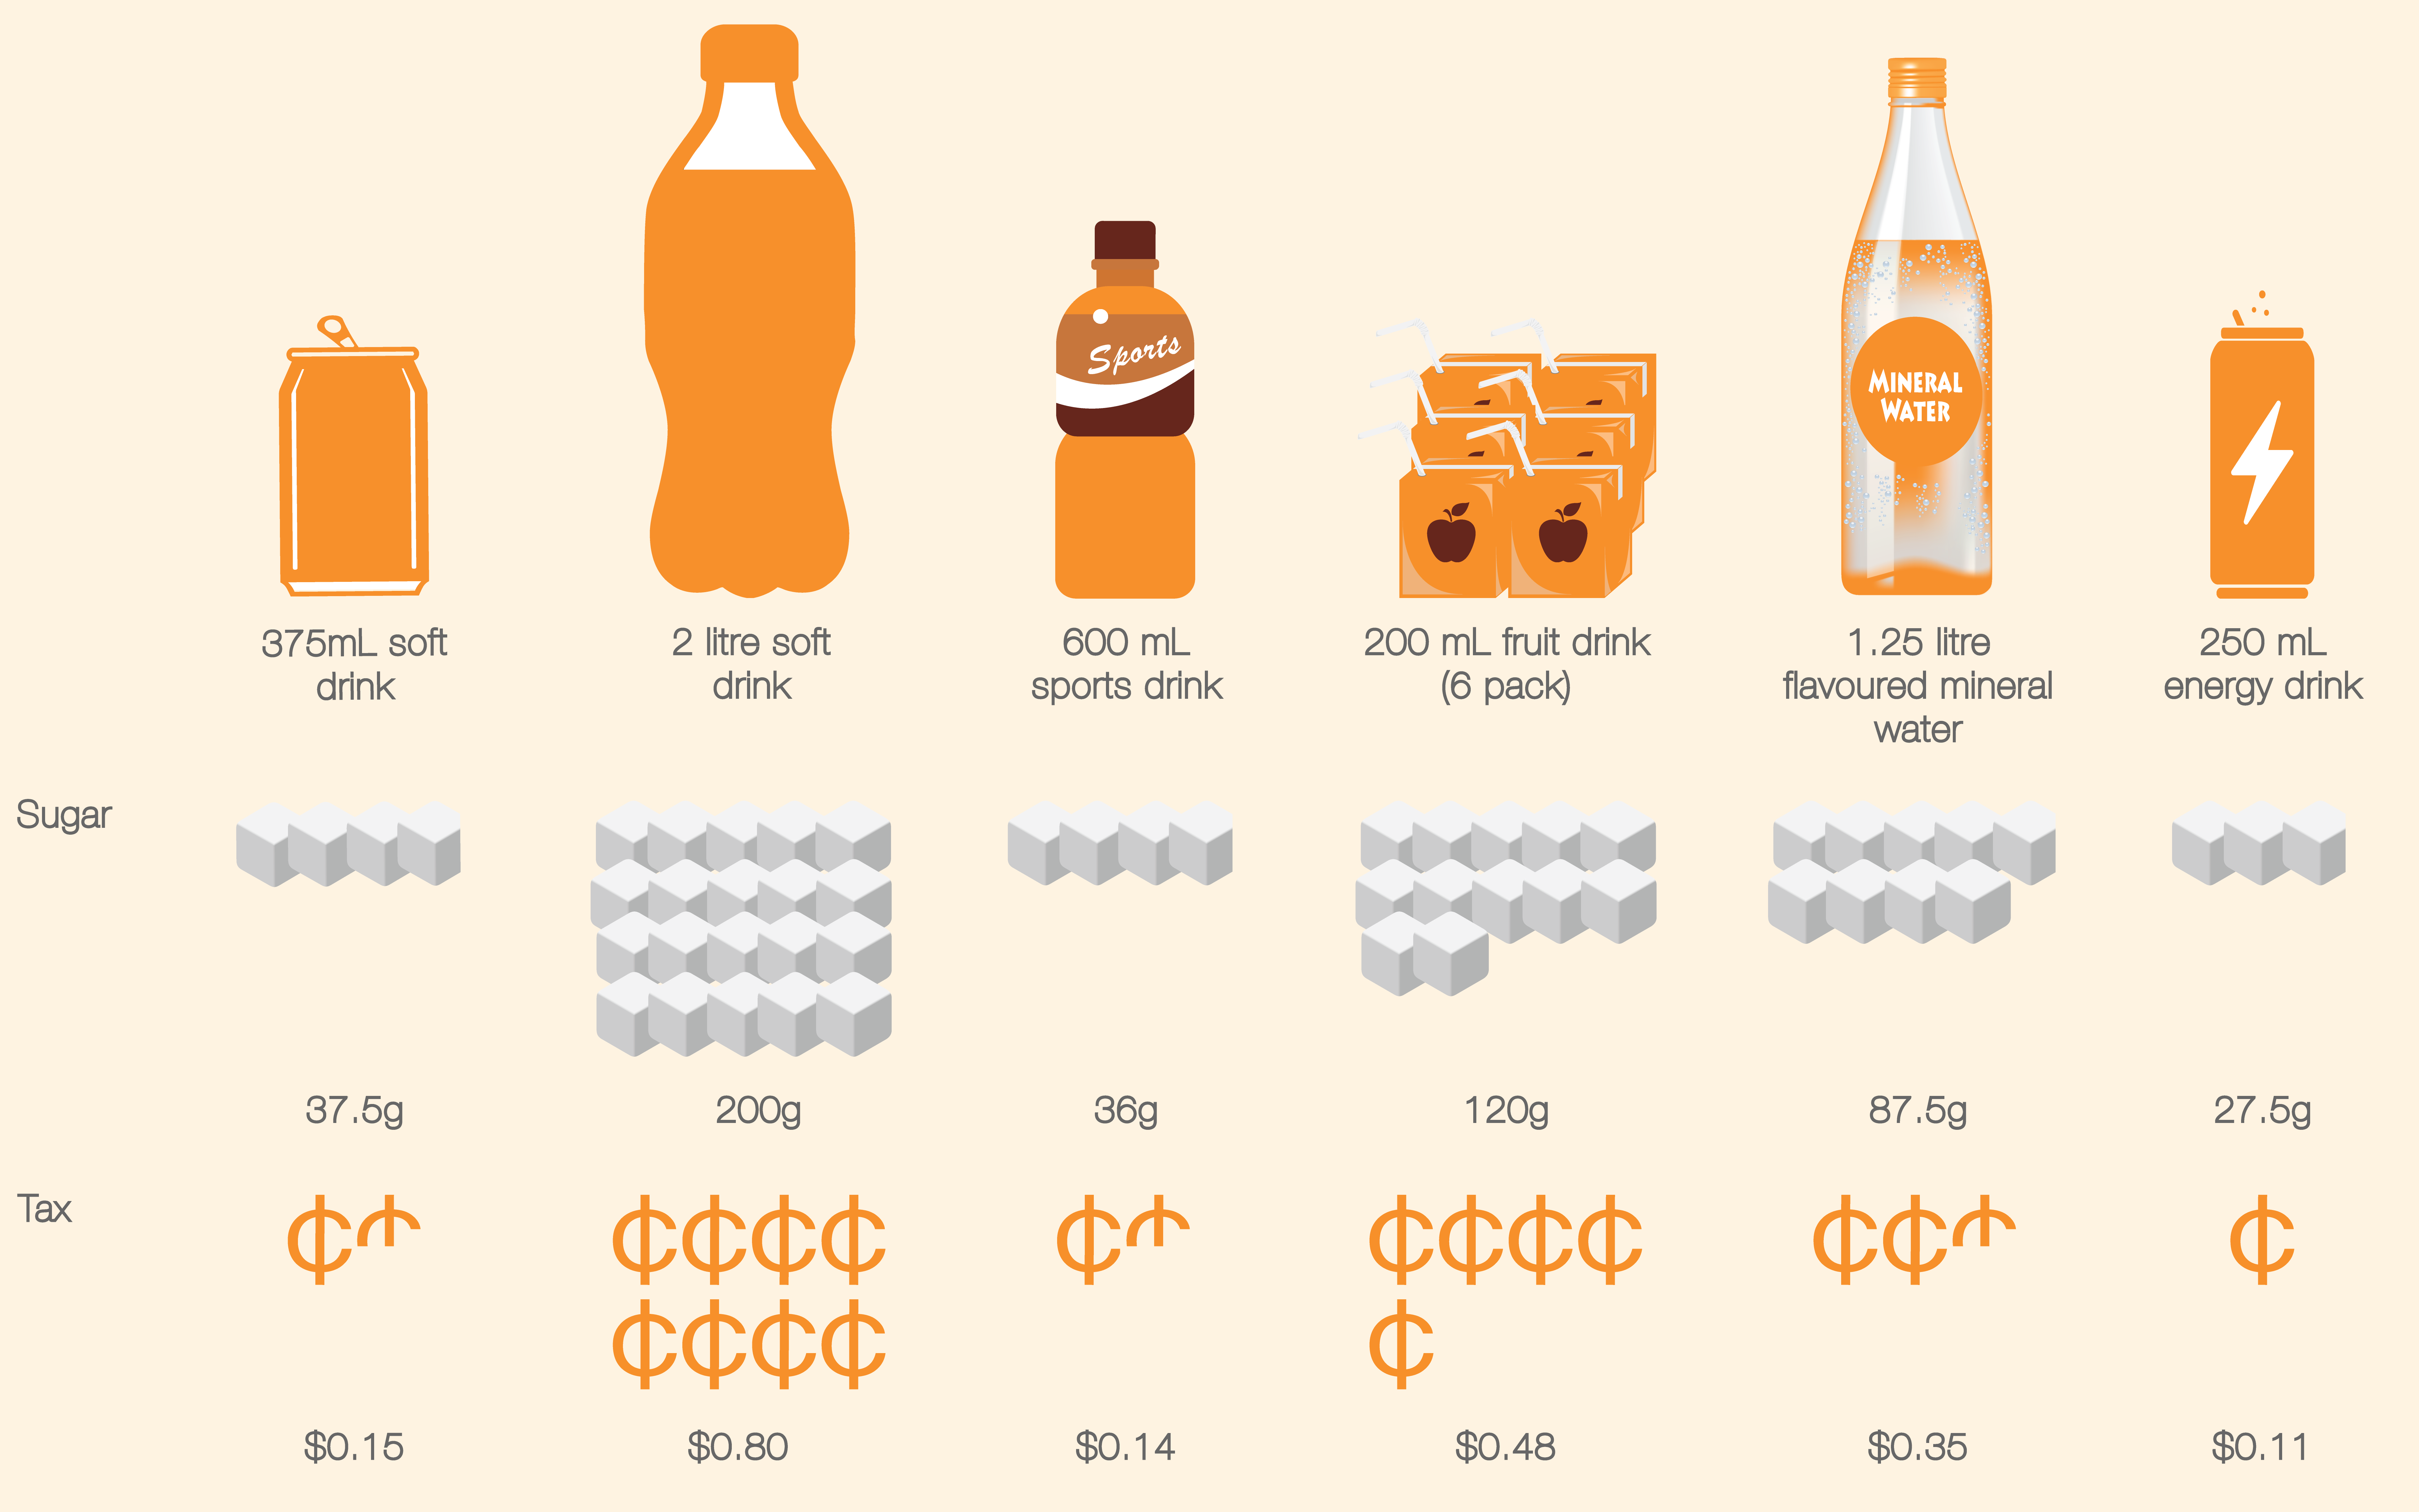
\includegraphics[width=.8\textwidth]{atlas/InfoGraphicSnip}

\source{Grattan analysis}
\end{figure}
\end{bigbox*}

\section{An excise tax will not be too difficult or expensive to administer}\label{an-excise-tax-will-not-be-too-difficult-or-expensive-to-administer}

An SSB tax would not be difficult to implement or overly expensive to administer.
SSBs would simply need to be defined and added to The Schedule in the \emph{Excise Tariff Act 1921}.
Manufacturers and distributors of SSBs would be required to obtain a licence from the ATO, as is the case with alcohol.%
\footnote{Applying a tax at the manufacturer level reduces complexity because fewer firms need to comply (\textcites{CnossenExcisetaxationAustralia}{Freebairn2010Taxationobesity})} The Parliamentary Budget Office estimates that the administrative costs of an SSB tax are about \$7 million a year, with a further \$7 million of set-up costs.%
\footnote{\textcite{Office2016PolicycostingAustralian}.
This costing was for a 20 per cent ad valorem excise, but administrative costs are likely to be similar for a volumetric excise tax or a sugar content excise tax.}


\section{Arguments against an SSB tax are overblown}\label{arguments-against-an-ssb-tax-are-overblown}

Unsurprisingly, the Australian beverage industry is strongly opposed to the introduction of an SSB tax.
The non-alcoholic beverages peak body, the Australian Beverages Council, has argued against the implementation of an SSB tax in the media and in submissions to government inquiries.%
\footnote{For example, the Australian Beverages Council submission to the NHMRC Australian Dietary Guidelines in 2012 (\textcite{Council2012AustralianBeveragesCouncil}), in response to the Greens 20 per cent SSB tax announcement (\textcite{Council2016Softdrinktax}).} The beverage industry's main arguments against an SSB tax are that it will be ineffective in combating obesity, it is regressive and that SSB (particularly soft drink) consumption is only a small proportion of energy intake and is falling.%
\footcite{Sharma2014effectstaxingsugarsweetened} We have addressed each of these arguments in this report. 

We acknowledge that an SSB tax is not a solution to the obesity problem on its own.
But an SSB tax will reduce consumption and partly reduce the third-party costs of SSB consumption which contributes to obesity.
We also acknowledge that the SSB tax impost is regressive.
But the tax burden is modest, there are similar untaxed healthier substitutes, and the health benefits are likely to be greatest for lower-income people.
Finally, while SSBs account for only a small proportion of “energy-in”, they are high in sugar, are absorbed quickly, can induce hunger and contain few or no valuable nutrients.

The processed food industry has a long history of aggressive lobbying against policies aimed at reducing consumption.%
\footcites{Nestle2015Sodapoliticstaking}{Observatory2016spoonfulsugarHow}{Koplan2010Responsefoodbeverage} In the US, the beverage lobby group spent millions unsuccessfully opposing the introduction of SSB taxes in Berkeley and Philadelphia, but successfully campaigned against other proposed SSB taxes in other cities and states.%
\footcites{Nestle2015Sodapoliticstaking}{Nadolny2016Sodataxpasses}{Organization2016FiscalPoliciesDiet}{Steinmetz2014BigSodaFights}{Nadolny2016Sodataxpasses}{Belluz2016UStaxes}


Job losses in the beverage industry will be minimal, and jobs will be created in other sectors of the economy as consumption patterns change.%
\footnote{Following the introduction of the Mexican SSB tax, employment in the beverage and energy-dense food sectors did not fall, and the overall unemployment rate did not increase (\textcite{SaludPublica2016Employmentchangesassociated})} There will likely be some switch to tap water, so overall demand for packaged beverages will likely fall only modestly.
However, as we have described, there will be a significant switch to artificially-sweetened beverages, which are also manufactured by SSB producers (for example, Coca-Cola Amatil produces Mt Franklin bottled water, the highest-selling bottled water brand in Australia).
This switch to non-sugar beverages will mean the reduction in total demand for beverages produced by Australian manufacturers will be minimal.
In addition, producers will reformulate products to reduce their exposure to the SSB tax.

The impact of an SSB tax on the sugar industry will also be minimal (see \Vref{box:impactSSBindustry}).

\begin{bigbox*}{The Australian sugar industry will face transition costs}{box:impactSSBindustry}

The Australian sugar industry produces 4-5 million tonnes~of raw sugar per year, of which 75-80 per cent is exported as bulk raw sugar.%
\footnote{This raw sugar is derived from 30-35,000 tonnes of sugar cane (\textcites{Canegrowers2015Statisticsfacts}{Agriculture2016SugarWorldMarkets}{Council2016Sugarcanestatistics}.} 95 per cent of Australia's sugar cane is grown in Queensland with the remainder grown in northern NSW.
In the past five years, Australia has accounted for 2-3 per cent of total world raw sugar production and 5-7 per cent of total world exports of raw sugar in recent years.%
\footnote{Australia's sugar production and consumption is projected to be flat at 5.0~million and 1.2~million tons, respectively, in 2016/17.
Exports are forecast to be higher at 3.9 million tons because trade agreements have increased access to markets such as South Korea (\textcite{Agriculture2016SugarWorldMarkets}).} The sugar industry employs around 16,000 people.%
\footcite{Council2016Sugarcanestatistics}

Australian SSB manufacturers use approximately 320,000 tonnes of Australian-produced sugar in their products (about 6 per cent of Australia's sugar production).
A reduction in SSB consumption will reduce demand for Australian produced sugar.
As a result, sugar industry groups have lobbied against the introduction of a tax on sugar.
However, an SSB tax will mainly result in more sugar being exported, rather than sold domestically, with a minimal impact on prices.

The estimated 15 per cent fall in SSB consumption in response to an SSB tax will result in a \textasciitilde{}50,000 tonnes reduction in demand for Australian sugar from domestic SSB manufacturers (\textasciitilde{}1 per cent of all sugar produced in Australia).
As manufacturers will likely pass on the SSB tax to retail prices in full, there should be minimal impact on the price received by sugar producers and cane growers.

The sugar that was previously sold to domestic SSB manufacturers will instead be exported rather than sold domestically.
As Australia only accounts for 5-7 per cent of total world exports and is a price-taker, increasing exports by \textasciitilde{}50,000 tonnes (\textasciitilde{}0.03 per cent of world production) would have a minimal impact on world prices, which are volatile and influenced by many global factors. 

An SSB will have some impacts though.
As Australia produces high-quality sugar, there will likely be additional costs to find new export markets.
Adjustment costs may also be localised.
For example, the NSW Sugar Milling Cooperation refinery at Harwood in northern NSW sells all of its produce into the domestic market, and may need to begin exporting.
These export difficulties and adjustment costs could be warrant a small government transition package.
\end{bigbox*}

\chapter{Using the sugar-sweetened beverages tax revenue }\label{using-the-sugar-sweetened-beverages-tax-revenue}

An SSB tax will raise substantial revenue for the Commonwealth Government, in the range of \$500~million a year depending on the design of the tax.
The government does not need to hypothecate the revenue from an SSB tax for a particular purpose.
However, identifying potential uses of the additional revenue may be politically useful to generate support for the introduction of the tax.%
\footnote{\textcites{Freebairn2010Taxationobesity}{Organization2016FiscalPoliciesDiet}{CnossenExcisetaxationAustralia}.
Although the hypothecation or `earmarking' of revenue from an excise tax can be politically useful, it is in practice irrelevant because the marginal expenditure decisions made by the government exist regardless of the source of the tax.}

\section{Additional spending on health or health research}\label{additional-spending-on-health-or-health-research}

We have predicated the SSB tax based on the third-party costs of obesity, most of which are borne by the government through higher health expenditure and foregone tax revenue.

The SSB tax revenue could be added to the health budget to improve primary care or hospitals.
The revenue could also be designated to preventative health measures or to the Medical Research Future Fund to research preventions and treatment of chronic diseases.

\section{Obesity prevention programs and interventions }\label{obesity-prevention-programs-and-interventions}

The SSB tax revenue could be spent on obesity prevention policies and interventions.
There is growing evidence that the best such interventions and policies have multiple elements or a `whole of systems' approach.%
\footnote{\textcites{Ewart-Pierce2016WholeCommunityObesity}{Health2016Insufficientphysicalactivity}{Hawkes2015Smartfoodpolicies}{Organization2016FiscalPoliciesDiet}{Roberto2012Factsfrontversus}{Mckinsey2014overcomingobesity}.
Randomised controlled trials are also underway to determine the effectiveness of different interventions in combating obesity in young children.
For example, the \textcite{Sobko2011randomisedcontrolledtrial} study which took place in Sweden.}

The WHO and public health advocates recommend improving access to healthy, unprocessed foods.
This can be done by subsidising healthy foods,\footcites{LordanShouldweput}{Organization2016FiscalPoliciesDiet} providing school breakfast/lunch programs, or other assistance to improve access to healthy foods in remote or disadvantaged areas.%
\footnote{\textcite{Organisation2015Usingpricepolicies} states that without intervention, `the prices of fruit and vegetables at point of purchase are likely to exceed the socially optimal price, and the quantity sold will be below the level needed for the maximum benefit to society'; \textcite{Kaplin2013Usingeconomicpolicy}.
Basic nutritious foods can be 30 per cent more expensive in rural areas(\textcite{Health2012Australiasfood}).
Access to affordable healthy foods is recognised as a problem in remote areas, especially among indigenous communities (\textcite{Thurber2014OverweightobesityIndigenous}).} The most effective policies to increase consumption of healthy alternatives are fruit and vegetable subsidies, and subsidised health foods at schools.%
\footcites{Kaplin2013Usingeconomicpolicy}{Organization2016FiscalPoliciesDiet}{Thow2014systematicrevieweffectiveness}{An2013Eatingbetterless}\footnote{There is evidence that combining taxes with subsidies for fruit and vegetables is effective at reducing population weight (\textcite{Organization2016FiscalPoliciesDiet}).} However, while subsidising healthy foods can increase consumption of targeted foods, thereby improving diet, subsidies can also increase overall energy intake.%
\footcites{Kaplin2013Usingeconomicpolicy}{Organization2016FiscalPoliciesDiet}{Cawley2015economyscalesselective}

School nutrition education programmes and other consumer education programmes are also effective in improving knowledge about healthy eating.%
\footcites{Research2007EvaluationNationalGo}{Capacci2012Policiespromotehealthy}{Ebbeling2002Childhoodobesitypublic}{Hawkes2013Promotinghealthydiets}{Hawkes2015Smartfoodpolicies}{Organization2016Reportcommissionending} There is strong public support for using the revenue from an SSB tax to reduce the price of healthy foods.%
\footcite{Morley2012Publicopinionfood}

Some policies and initiatives that are generally regarded as an important part of efforts to combat obesity, such as restricting food marketing to children, require changes to laws and regulations, not government spending.%
\footnote{For example, processed food advertising has been banned or limited in countries such as Norway, Sweden and South Korea (\textcite{Cawley2015economyscalesselective}).}

\begin{verysmallbox}{Other jurisdictions with an SSB tax have allocated the revenues to children}{SSBJurisdictionRevenue}

To increase the public's acceptance of an SSB tax, some jurisdictions have devoted the revenue raised to children's education and childhood obesity prevention policies.
For example, Philadelphia City Council plans to use the revenue from its soda tax to expand early childhood education programs and improve parks and recreation centres in the city.%
\footcite{Nadolny2016Sodataxpasses} The UK government intends to spend the revenue from the proposed SSB tax on physical activity and healthy eating programs for school-aged children.%
\footcite{HMTreasurysugarlevy} Some of the revenue from Mexico's soft drink and fast food tax has been used to install water fountains in schools in disadvantaged areas.%
\footcite{Soares2016Puttingtaxesdiet}
\end{verysmallbox}

\section{Reducing Australia's budget deficit}\label{reducing-australias-budget-deficit}

Finally, the Commonwealth Government could use the SBS tax revenue to reduce the budget deficit, forecast to be \$37.1 billion in 2016/17.%
\footcite{Treasury2016201617BudgetBudget}

\begin{bigbox*}{Key findings and recommendations}{key-findings-and-recommendations}

\begin{itemize}
\item
  The prevalence of obesity has increased significantly over the past few decades.
In 2014/15, 28 per cent of adult Australians were obese.
\item
  Obesity imposes significant personal and third-party costs.
Third-party costs, primarily borne by governments, include higher healthcare spending, higher welfare spending and lower tax revenue due to lower employment rates.
We estimate that the third-party costs of adult obesity in 2014/15 were \$5.3~billion.
\item
  Many factors are contributing to the rising prevalence of obesity in Australia.
But the primary cause is excessive consumption of unhealthy processed food.
This is driven by `market failures', including consumers having a limited understanding of processed foods and behavioural factors that can limit self-control, and people not bearing the full costs of over-consumption of unhealthy foods.
\item
  The Commonwealth Government use tax measures to reduce the third-party costs created by the excess consumption of energy-dense, nutritionally poor foods that contribute to obesity.
\item
  An excise tax on the sugar contained within SSBs is the best, and simplest, tax option to recoup some of the third-party costs generated by obesity.
However, an SSB tax by itself will not solve Australia's obesity problem.
\item
  SSBs that should be subject to a tax are non-alcoholic, water-based drinks with added sugar.
This includes soft drinks, flavoured mineral waters, energy drinks, cordials and fruit juices with added sugar.
\item
  The SSB tax should be about 40 cents per 100 grams of sugar contained within SSBs.
This will increase the price of a 2 litre bottle of soft drink by about 80 cents.
The second-best alternative is a tiered excise tax based on the volume of liquid per SSB.
\item
  An SSB excise tax as described will generate around \$500~million in annual revenue to recoup the third-party costs of obesity, reduce consumption of SSBs by about 15 per cent by increasing the retail price and lead to a slight reduction in the prevalence of obesity.
\item
   About 80 per cent of Australia's sugar production is exported.
An additional 1 per cent of Australia's annual sugar production will need to be exported due to the suggested SSB tax, and this may mean transition assistance is required for the millers affected.
\item
  The revenue from an SSB tax could be used to reduce the Commonwealth Government's budget deficit, be spent on healthcare or be spent on obesity prevention programs and interventions.
\end{itemize}
\end{bigbox*}

\appendix

\onecolumn
\chapter{SSB tax literature review summary}\label{appendix-1-ssb-tax-literature-review-summary}

\bgroup
\def\arraystretch{1.6}
\LTXtable{\textwidth}{tables/SSB-studies-Australia-modelling-meta-analysis}
\clearpage
\LTXtable{\textwidth}{tables/SSB-studies-Overseas-evaluation}
\clearpage
\LTXtable{\textwidth}{tables/SSB-studies-Overseas-modelling-meta-analysis}
\egroup




\begin{table}[t]
\caption{Summary of studies on pass through of SSB taxes to retailers}

\bgroup
\def\arraystretch{1.5}
\begin{tabularx}{\textwidth}{Xp{5cm}p{5cm}p{10cm}}
\toprule
\textbf{Authors} & \textbf{Study details} & \multicolumn{1}{p{5cm}}{\textbf{Elasticities} / 

\textbf{effect on consumption}} & \textbf{Pass through} \\
\cmidrule(lr){1-4}
Berardi \emph{et al.} (2016) & Evaluation of French soft drink tax on consumer prices & & Tax fully shifted to soda, almost fully shifted to fruit drinks, incomplete to flavoured waters (6 months after introduction) \\
Grogger (2015) & Evaluation of Mexico's SSB tax using Mexico's Consumer Price Index & & The SSB excise tax of \textasciitilde{}8-10 percent raised the price of regular soda by 12 per cent \\
Bonnet and R\'equillart (2013), & Modelled the effects of an ad valorem and excise tax on French retail soft drink prices & & Retailers passed on to consumers between 60 and 90 per cent of the ad-valorem tax increase, and between 110 and 130 per cent of the excise tax \\
Bergman and Hansen (2010) & Evaluation of Denmark excise tax & & The increase in soft drink excise tax was on average over-shifted, although many retailers did not increase their price at all \\
Bahl \emph{et al.} (2003) & Evaluation of Ireland's soft drink tax levied in the 1970s to the early 1990s & The estimated price elasticity of demand for soft drinks = --1.10 & Under-shifting of tax to retail prices \\
\bottomrule
\end{tabularx}
\egroup

\end{table}
\twocolumn

\chapter{Estimating the third-party costs of obesity }\label{appendix-2-estimating-the-third-party-costs-of-obesity}

The third-party costs of obesity calculated in this report are based on the methodology used in \citeauthor{PwC2015Weighingcostobesity}'s \citeyear{PwC2015Weighingcostobesity} report \citetitle{PwC2015Weighingcostobesity}.

We estimate the additional costs incurred by obese people relative to people in the normal BMI range.
The additional costs incurred by governments are considered third-party costs because they are paid for by higher taxes.

The most recent obesity data is from the ABS National Health Survey: First Results 2014/15 (\Vref{tbl:Adult-obesity-estimates}).%
\footnote{PwC calculates costs in 2011/12 and inflates this to 2014/15 dollars.}

\begin{table}
\caption{Adult obesity estimates}\label{tbl:Adult-obesity-estimates}
\units{18+, 2014/15, by obese class (BMI)}

\bgroup
\def\arraystretch{1.2}
\begin{tabular}{lrr}
\toprule
\textbf{Category} & \textbf{BMI\phantom{+}} & \textbf{Number} \\ 
\midrule
Class I & 30-34.99\phantom{+} & 3,251,000 \\
Class II & 35-39.99\phantom{+} & 1,120,000 \\
Class III & 40+ & 572,000 \\
 & \\[-10pt] 
\textbf{Total} & & \textbf{4,944,000} \\
\bottomrule
\end{tabular}
\egroup

\source{\textcite{ABS20164364055011AustralianHealth}}
\end{table}

\section{The third-party costs of obesity}\label{the-third-party-costs-of-obesity}

We estimate that the third-party costs of obesity in 2014/15 were \$5.3~billion dollars (\Vref{tbl:3rd-party-costs-of-adult-obesity}).

\begin{table}
\caption{Third-party costs of adult obesity in 2014/15}\label{tbl:3rd-party-costs-of-adult-obesity}
%\units{\$billions, 2014/15 dollars}

\bgroup
\def\arraystretch{1.2}
\begin{tabular}{lc}
\toprule
\textbf{Category} & \multicolumn{1}{p{2.8cm}}{\centering\textbf{Third-party costs}} \\ \cmidrule(lr){1-2}
GPs, specialists, allied health & \$0.6b \\
Hospital care & \$0.6b\\
Pharmaceuticals & \$1.4b \\
Foregone tax & \$2.3b\\
Additional welfare & \$0.4b\\ \cmidrule(lr){1-2}
\textbf{Total} & \textbf{\$5.3b} \\
\bottomrule
\end{tabular}
\egroup

\notes{Foregone tax includes foregone income tax from lower employment rates, and foregone company tax from absenteeism and presenteeism.
Welfare includes additional disability support pension and Newstart allowance payments.}
\source{Source: \textcite{PwC2015Weighingcostobesity}, Grattan analysis}
\end{table}

\subsection{GP, specialists and allied health costs}\label{gp-specialists-and-allied-health-costs}

Additional GP, specialists and allied health costs were estimated to be \$595~million in 2014/15.
Additional costs are based on additional excess costs for medical services (GP visits, allied health services and specialists) for obesity class I, II and III patients estimated by \textcite{Colagiuri2010costoverweightobesity}.%
\footnote{Unpublished data from \textcite{Colagiuri2010costoverweightobesity}, obtained from author.
Originally in 2004/05 dollars.
Excess costs are assumed to be government costs.}.
These excess costs were inflated by the health cost index calculated by the Australian Institute of Health and Welfare.%
\footnote{\textcite{Health2015HealthexpenditureAustralia}, Table C2.
Health costs increased by 27.9 per cent between 2004/05 and 2014/15.}

The excess costs for GP visits, allied health services and specialists for the obese class I, II and III categories were multiplied by the number of people in each obesity category in 2014/15 (\Vref{tbl:Adult-obesity-estimates}).

The calculated excess costs due to obesity for each medical service, in 2014/15 dollars, were \$226~million for GP services, \$123 for allied health service and \$246~million for specialists.

\subsection{Hospital care }\label{hospital-care}

The additional spending per obese person on inpatient, outpatient and emergency hospital treatment compared to those in the normal BMI range was calculated by PwC from a variety of sources.%
\footcite[][48]{PwC2015Weighingcostobesity} Costs were split by age groups (18-44 and 45+) and obesity class (I, II and III).
These estimates were multiplied by the number of people in each obesity class that had a hospital episode.%
\footnote{Obtained from Australian Health Survey: Health Service Usage and Health Related Actions, 2011/12 (\textcite{ABS20134364055002AustralianHealth}).} Total additional costs were calculated to be \$1.2~billion.

PwC estimate that 51 per cent of the total additional cost of hospital care due to obesity is borne by Commonwealth and state governments.%
\footnote{The remainder is assumed to be covered by private health insurers and individuals.} This proportion was applied to the total additional cost estimate, resulting in an estimate of the third-party costs attributable to hospital care of \$628~million.

\subsection{Pharmaceuticals }\label{pharmaceuticals}

An estimated 74 per cent of obese class I and 78 per cent of obese class II and III use pharmaceuticals.%
\footcite{Buchmueller2015Obesityhealthexpenditures} Pharmaceutical costs are subsidised by the Commonwealth Government through the Pharmaceutical Benefits Scheme.

Obese class I, II and III were split by age into two age groups, 18-44 and 45+.
Additional spending on obese people aged 45+ relative to people of normal weight on pharmaceuticals was derived from \textcite{Buchmueller2015Obesityhealthexpenditures}.
Pharmaceutical costs for 18-44 year olds were estimated to be 34 per cent of costs for the older age group.%
\footcite[][50]{PwC2015Weighingcostobesity}

Using these assumptions, the estimated additional pharmaceuticals costs incurred by the Commonwealth Government due to obesity in 2014/15 was estimated at \$1.38~billion.

\subsection{Foregone tax}\label{foregone-tax}

\subsubsection{Lower employment rates}

The employment rate among obese people was 65 per cent in 2011/12, 4.7 percentage points lower than people in the normal BMI range.%
\footcite{ABS2013436405503AustralianHealth} The employment rate among obese class III individuals is estimated to be 1.5 percentage points lower than obese class I and II.%
\footnote{\textcite[][59]{PwC2015Weighingcostobesity}, `This corresponds with the proportion of obese type III individuals estimated to claim disability pensions based on Department of Social Services claims totals for relevant disease categories, adjusted for per cent of these categories with obesity co-morbidities and relative risk from obesity'.}

Employment rates for obese class I and II individuals were therefore calculated to be 65.2 per cent, and 63.7 per cent among obese class III individuals.
We assume that obesity contributes to lower employment rates, which reduces income tax received by the Commonwealth Government, based on recent studies which generally conclude that obesity results in poorer labour market outcomes.%
\footnote{\textcite{Boeckerman2016EffectWeightLabor} find that higher BMI reduces employment and increases social welfare payments. \textcite{Reichert2015Obesityweightloss} finds a positive employment effect of weight loss for women. \textcite{Rooth2009Obesityattractivenessdifferential} finds that obese women are less likely to receive a call-back for an interview after a CV appraisal. \textcite{Cawley2015economyscalesselective} also summarises the literature and finds that obesity worsens employment prospects.~However, there are some findings that unemployment contributes to obesity and other unhealthy behaviours \textcites{Schmeiser2009Expandingwalletswaistlines}{Marcus2014Doesjobloss}.}

We assume that unemployed obese people would receive 9 per cent less than average earnings if employed due to lower education among obese people (on average).%
\footnote{For example, 12 per cent of obese adults hold a Bachelor’s degree compared to 22 per cent with a normal BMI \textcite{ABS20164364055011AustralianHealth}).
The 9 per cent reduction was estimated using the earnings premium from \textcite{Norton2012MappingAustralianhigher} and education levels from \textcite{ABS2013436405503AustralianHealth}. \textcite{Kortt2010Doessizematter} find no significant relationship between BMI and hourly wages among Australian adults, controlling for a variety of factors such as years of education, whether born overseas, age and father’s occupational status.
This suggests there is no weight discrimination by Australian employers.
Overseas studies generally find that a higher BMI is associated with lower wages, particularly for women, controlling for other factors (see \textcites{Cawley2004impactobesitywages}{Cawley2005comparisonrelationshipobesity}).}  Obese people are less likely to hold a university degree or other tertiary qualification than people with a BMI in the normal range.
The average annual total private sector earnings in 2014/15 was \$56,641, with expected earnings for an obese person estimated to be \$51,602.%
\footnote{This is the average of November 2014 and May 2015 seasonally adjusted private sector total earnings, multiplied by 52 (\textcite{ABS201663020AverageWeekly}, Table 5).
We use earnings for all workers, rather than average earnings for full-time workers used by PwC.}  

Using the 2014/15 personal income tax rates, the average tax paid was \$9,955, plus the 2 per cent Medicare levy (\$1,133) (a total of \$11,088).
This foregone tax on average earnings was multiplied by the 232,000 obese people that we assume would be employed if employment rates for obese people were the same as for people in the normal BMI range, resulting in total foregone income tax of \$2.17~billion.

\subsubsection{Absenteeism and presenteeism}

Absenteeism and presenteeism reduce firm profits through higher labour costs and lower productivity.
Lower profits flow through as a cost to the government through lower company tax receipts.

We estimate that the third-party costs from lower company tax revenue due to absenteeism are minimal.
We use the assumption that obese people were absent from work on average 4 hours more per year than non-obese people,\footcite[][55]{PwC2015Weighingcostobesity}, based on \textcite{ABS20134364055002AustralianHealth}.
The employment rate for obese people was 65 per cent,\footcite{ABS2013436405503AustralianHealth} 19 per cent of workers are casual workers\footcite{ABS201563333} (so don't receive wages if sick) and average ordinary time earnings per hour in 2014/15 were \$38.80.%
\footcite{ABS201663020AverageWeekly} Using these assumptions, the additional wages paid by employers to workers absent due to obesity was estimated to be \$400~million.
As firms face higher labour costs and therefore reduced profits, government revenue from company tax is reduced by \$121~million (using a 30 per cent company tax rate).
However, these workers pay income tax on these earnings (through sick leave).
So there is only a small net reduction in government revenue.
We assume that 30 per cent of the \$121~million in lost company tax revenue is not offset by income tax receipts from workers, resulting in absenteeism costing the government \$36~million in revenue.

Low productivity at work due to poor health or other reasons is known as presenteeism.
Presenteeism due to obesity increases labour costs.
PwC estimate that obese workers are 0.23 per cent less productive at work due to co-morbidities related to obesity (diabetes, heart disease, hypertension, cancer and back/neck problems).%
\footcite[][56]{PwC2015Weighingcostobesity} There were 3.2 million obese workers in Australia in 2014/15, with average annual private sector earnings of \$56,641.%
\footcite{ABS201663020AverageWeekly} This results in lost productivity worth \$418~million in 2014/15.
We conservatively estimate that half of this productivity loss is a cost to firms, which reduces company tax revenue by \$63~million in 2014/15.

\subsection{Welfare}\label{welfare}

PwC estimate that 1.5 per cent of obese class III individuals are on the Disability Support Pension (DSP).
In January 2015, the DSP was worth \$20,665 per year.%
\footnote{The maximum basic rate DSP for a single person} We assume that 80 per cent of people on the DSP could gain employment if they were not obese, so additional DSP payments by the Commonwealth Government in 2014/15 were estimated to be \$142~million.

Commonwealth Government unemployment assistance payments (the Newstart Allowance) are higher than would be the case if there was no obesity, because obesity contributes to lower employment rates (see `Foregone tax'). \textcite{Colagiuri2010costoverweightobesity} calculate that obesity class III people receive an average of \$438 (2014/15 prices) more Newstart Allowance payments per person than normal weight and overweight people.%
\footnote{\textcite{Colagiuri2010costoverweightobesity} estimate that obese class I and II people receive slightly less unemployment benefits than people with BMI in the 19-29.9 range.
This difference is ignored.} There were 572,000 obese class III people in 2014/15, resulting in total excess Newstart Allowance payments of \$250~million.

Summing these two forms of welfare gives an estimated \$392 million in additional welfare payments in 2014/15.%
\footnote{\textcite{Boeckerman2016EffectWeightLabor} find that a higher BMI is associated with a higher chance of receiving social assistance.}

\section{Additional third-party costs of obesity }\label{additional-third-party-costs-of-obesity}

\subsubsection{Deadweight loss from higher taxes}\label{deadweight-loss-from-higher-taxes}

Raising taxes is not costless.
All taxes distort decision making, reducing efficiency and economic output.%
\footnote{\textcites[][Box~1]{Daley2015Propertytaxes}{Freebairn2010Taxationobesity}} To generate the additional \textasciitilde{}\$3~billion in taxes to pay for the additional health costs and welfare spending (ignoring the foregone tax revenue due to obesity), assuming a marginal excess burden of 25 cents for each dollar of tax raised, would result in a deadweight loss of \$750~million.

\subsubsection{Higher private health insurance premiums}\label{higher-private-health-insurance-premiums}

Private health insurers cover the higher expected medical costs of obese people by charging higher premiums for all policyholders.
These higher premiums are paid by all people with private health insurance due to the `community rating' principle that requires insurers to charge all people the same premium, regardless of age or health.%
\footnote{In the US, employers can charge obese workers higher premiums if they decline to participate in a wellness program, such as those to promote healthy weight (\textcite{Karnani2016ObesityCrisisas}).} As a result, non-obese people have higher private health insurance premiums than if there was no obesity.%
\footnote{In addition to this transfer from non-obese to obese people, there is also the possibility of an additional externality arising from people behaving differently since they know they are covered by insurance.
This `moral hazard' is more important in countries such as the US where there is no universal public healthcare system (\textcite{Bhattacharya2011Whopaysobesity} and \textcite{Botkins2015DoesHealthInsurance}).
Some of the cost of higher insurance premiums is absorbed by the Commonwealth Government through the means-tested private health insurance rebate (expenditure on the rebate was just under \$6~billion in 2014/15).}

\subsubsection{Costs of childhood obesity}\label{costs-of-childhood-obesity}

The third-party costs of obesity calculated above do not include the costs of childhood obesity.
However, the third-party costs of childhood obesity are likely to be fairly small because prevalence rates are lower and there are no tax revenue losses from lower employment rates and extra welfare payments).
Health costs would also be much lower due to lower rates of chronic diseases among children.

Lifetime costs arising from childhood obesity are significant because obese children are more likely to become obese adults.%
\footcites{Health2013AustralianDietaryGuidelines}{Baker2007Childhoodbodymass}{Summerbell2005Interventionspreventingobesity}{Popkin2004nutritiontransitionworldwide}


\subsubsection{Government spending on obesity campaigns and interventions}\label{government-spending-on-obesity-campaigns-and-interventions}

The Commonwealth Government spends money on public interventions and campaigns to reduce obesity rates, estimated to be \$60 million in 2014/15.%
\footnote{PwC estimated that \$154 million would be spent on preventative health, but in the 2014/15 Budget it was announced that this would be discontinued, saving \$90~million each year. \textcites{PwC2015Weighingcostobesity}{Treasury2016201617BudgetBudget}.} State governments also spend significant amounts on obesity prevention campaigns, advertising and interventions.%
\footnote{\textcite{PwC2015Weighingcostobesity} estimated that state governments spent an additional \$390~million on health care due to obesity}

\chapter{Modelling sugar-sweetened beverages tax options}\label{appendix-3-modelling-sugar-sweetened-beverages-tax-options}

\subsubsection{SSB consumption and sales revenue data}\label{ssb-consumption-and-sales-revenue-data}

SSB industry sales data was used to calculate revenue from a hypothetical SSB tax and changes in SSB consumption in 2017.
SSBs were defined as non-alcoholic, water-based beverages with added sugar.

Using data from IBISWorld and Retail World, total SSB sales were calculated to be 1.62 billion litres (\$3.31 billion in revenue) in 2015.%
\footnote{\textcites{Media2015RetailWorldAnnual}{IBISWorld2016FruitJuiceDrink}{IBISWorld2016SoftDrinkManufacturing}.
According to Retail World data, drinks with added sugar account for 52 per cent of the volume of beverages sold.} 
This estimate aligns with the \textcite{Levy2014QuenchingAustraliasthirst} estimate of SSB sales of 1.62 billion litres in 2011 (as there has been modest growth in SSB volumes in recent years) and ABS data from 2011/12.%
\footnote{By multiplying average consumption of SSBs per person and the population \textcite{ABS20144364055007AustralianHealth}}

Volume growth of 0.4 per cent from 2014 to 2015\footcite{Media2015RetailWorldAnnual} was used to forecast volume growth in 2017.
Using this assumption, projected SSB sales was forecast to be 1.64~billion litres in 2017.

\subsubsection{SSB tax options}\label{ssb-tax-options}

Four SSB excise tax options were modelled, with different tax rates modelled for each tax type:

\begin{itemize}
\item
  A tax on the sugar content of SSBs
\item
  A tax on the volume of SSBs (\eg~30 cents per litre) (a volumetric tax)
\item
  A tax on the volume of SSBs, with escalating rates (a tiered/escalating volumetric tax)
\item
  An ad valorem excise tax (\eg~a tax of 20 per cent on the retail price of SSBs)
\end{itemize}

\subsubsection{Calculating SSB tax revenue -- the key assumptions }\label{calculating-ssb-tax-revenue-the-key-assumptions}

SSB tax revenue estimates were done for 2017. 2017 sales and consumption forecasts were done for a scenario with no SSB tax, and compared to a scenario with different SSB taxes.

The key assumptions were:

\begin{itemize}
\item
  Average price of SSBs estimated to be \$2.00 per litre in 2017 for aggregate estimates (\$2.04 in 2015).\footnote{The average price per litre for SSBs in 2015 was calculated by dividing total sales value over volume, giving an average price of \$2.04 per litre.
Because water-based, non-alcoholic beverages prices have fallen in recent years, and this is expected to continue, the average price of SSBs is forecast to be \$2 per litre in 2017.} Category prices for market segments (\eg~soft drinks, juices, iced tea) were used for tax estimates calculated by summing market segments and the escalating volumetric SSB tax.
\item
  Excise tax fully passed on to retail price\footnote{The evidence from SSB excise taxes introduced overseas is that taxes are fully or over-shifted and that excise taxes are passed on to consumers quickly}
\item
  Price elasticity of demand for SSBs of \(-0.9\) for aggregate estimates.
Category elasticities for market segments (\eg~soft drinks, juices) were used for tax estimates calculated by summing market segments and the escalating volumetric SSB tax.%
\footnote{Elasticities for SSB categories were obtained from \textcite{Sharma2014effectstaxingsugarsweetened} and \textcite{Zhen2014Predictingeffectssugar}, and ranged from \(-0.63\) for soft drinks to \(-2.36\) for sports and energy drinks.
Substitution across categories, using cross-price elasticities, was not included in the model.
Cross-price elasticity estimates differ significantly between studies \textcite{Organization2016FiscalPoliciesDiet}).
A general finding is that the cross-price elasticity between SSBs and artificially-sweetened beverages is positive, which means they are substitutes.
Bottled water and SSBs are also found to be substitutes.}
\item
  Average sugar content of SSBs = 9.27 grams/100mL in 2017, unchanged from current level (this assumes no immediate product reformulation in response to the tax).%
\footnote{Weighted average of sugar content using sub-categories of SSBs (soft drinks (cola and non-cola), fruit juice/drinks, energy drinks, cordial, mixers, sports drinks, flavoured mineral waters, iced tea) \textcites{rethinksugarydrink2016Howmuchsugar}{HealthCth2014FactSheetHow}} 
\item
  GST effects ignored\footnote{GST revenue may increase slightly due to an SSB excise tax}
\end{itemize}

\subsubsection{Calculating SSB tax revenue -- the results }\label{calculating-ssb-tax-revenue-the-results}

\begin{table}
\caption{Possible SSB taxes raise \$400-600~million in revenue and reduce SSB consumption}
\units{2017}

\input tables/SSBTaxOptions
\notes{Tiered volumetric tax is 20c/litre on SSBs with sugar content \textless{}8g/100mL; 40c/litre sugar content \textgreater{}8g/100mL}

\source{Grattan analysis}
\end{table}

Projected consumption in 2017 with an SSB tax was calculated by subtracting the change in quantity due to the excise tax from projected consumption in 2017 with no SSB tax.%
\footnote{\(\% \Delta \text{quantity due to tax} = \% \Delta \text{price} \times \text{price elasticity of demand}\).} 
Total tax revenue was then obtained by multiplying the projected consumption with an SSB tax by the tax rate.%
\footnote{For the sugar content tax, this was the tax rate by the amount of sugar consumed within SSBs.
For the volumetric tax, this was the projected consumption in litres multiplied by the tax rate.
For the ad valorem tax, this was the projected total revenue multiplied by the tax rate.}

Tax revenue from the \$0.20/\$0.40 tiered volumetric SSB tax option was estimated by creating high sugar content (more than 8 grams of sugar per 100mL) and low sugar content (less than 8 grams of sugar per 100mL) SSB groups.%
\footnote{The volume of high-sugar SSBs was estimated to be 1.35~billion litres (83 per cent share) and the volume of low sugar SSBs was estimated to be 0.29~billion litres (17 per cent share). 20 per cent of non-cola soft drinks and 20 per cent of fruit juices/drinks were assumed to be low-sugar, as were all cordials, sports drinks and iced teas.} Category price elasticities were used to calculate changes in consumption. \$430~million of the \$480~million in tax generated by the tiered volumetric tax was from the high sugar drinks (sugar content \textgreater{}8g/100mL).

For each SSB tax option, total SSB tax revenue was also calculated by summing the tax generated by SSB sub-categories to compare with the aggregate SSB tax estimate.%
\footnote{The SSB categories used were: soft drinks (cola and non-cola), fruit juice/drinks, energy drinks, cordial, mixers, sports drinks, flavoured mineral waters, iced tea.
Volumes were estimated using the same approach to gross-up the aggregate sales of SSBs: \textcites{IBISWorld2016SoftDrinkManufacturing}{IBISWorld2016FruitJuiceDrink}{Media2015RetailWorldAnnual}.
The share of sugar-free/diet drinks within each category were obtained from \textcite[][Table~1]{Levy2014QuenchingAustraliasthirst}.
If no evidence was available, the proportion of sales within a category that contained added sugar was estimate (\eg~that 80 per cent of non-cola soft drinks and fruit juices contain added sugar).
Cross-category substitution was not considered} Summing the revenue generated within each SSB sub-category yielded very similar results to the aggregate SSB tax calculations for all SSB tax options (within 2-4 per cent of the aggregate estimate).

\printendnotes
\printbibliography

\end{document}
